\section{Описание практической части}
\label{sec:Chapter4} \index{Chapter4}

В это разделе описываются все проведенные эксперименты, а также их результаты. Важно отметить, что все вставляемые фрагменты кода используют библиотеки PyTorch \cite{pytorch}, RDKit \cite{RDKit} и HuggingFace \cite{huggingface}, а также предполагают наличие определенных глобальных переменных и конфигураций, которые не указаны в коде.


\subsection{Препроцессинг данных}
Препроцессинг данных начинается с использования библиотеки RDKit \cite{RDKit} для преобразования строковых представлений молекул в формате SMILES в структурированные графовые объекты. Это позволяет перевести химическую информацию, содержащуюся в SMILES, в формат, который может быть эффективно обработан современными графовыми нейронными сетями.

\begin{enumerate}
    \item Импорт необходимых модулей из библиотеки RDKit, определение списков атомов, хиральности и типов связей (были взяты стандартные списки из RDKit).
    
    \item Создание функции \texttt{get\_graph\_columns}, которая принимает SMILES-строку и возвращает графовое представление молекулы (матрицу связей, признаки узлов, рёбер, а также количество узлов в графе).
    
    \item Применение функций RDKit для преобразования SMILES в объект молекулы, из которого затем извлекается информация об атомах и связях для создания графового представления.
    
    \item Построения матрицы признаков узлов графа (для чего используются кодирование атомных номеров, хиральностей и типов связей).
    
    \item Применение функции \texttt{get\_graph\_columns} к стоблцу датасета, содержащему SMILES.
\end{enumerate}

Этот процесс позволяет преобразовать большое количество молекул, представленных в виде SMILES, в структурированные графовые данные для предсказания молекулярных свойств с помощью GNN. 

Данный препроцессинг производится над датасетом ChemBL \cite{ChemBL}, где содержатся также необходимые отпечатки молекул, которые будут использоваться как вход для трансформера.


\subsection{Обучение RoBERTa}
Обучение модели RoBERTa для задач хемоинформатики требует специальной настройки и адаптации стандартных процедур обучения трансформеров. В этом разделе описывается процесс настройки токенайзера, методика обучения с маскированием и тестирование обученной модели, а также анализ полученных результатов.

\subsubsection{Настройка токенайзера}
Используя библиотеку HuggingFace \cite{huggingface}, был создан ByteLevelBPETokenizer. Процесс настройки включает в себя следующие этапы:

\begin{enumerate}
    \item Обучение токенайзера на полученных файлах с целью создания словаря токенов и правил их слияния. Параметры обучения включают размер словаря, минимальную частоту токенов и специальные токены ($<s>, <pad>, </s>, <unk>, <mask>$).
    
    \item Сохранение обученного токенайзера, включая файлы \texttt{vocab.json} и \texttt{merges.txt}, которые содержат информацию о словаре токенов и правилах слияния.
    
    \item Тестирование токенайзера на примере молекулярной последовательности для проверки корректности токенизации и присвоения идентификаторов токенам.
\end{enumerate}
Токенайзер позволяет уменьшить размер словаря. Это позволяет снизить размерность пространства наших значений хеш-функции (используемой в алгоритме ECFP) с $2^{32}$ до размерности пространства токенов (примерно 10000).

\subsubsection{Обучение маскированием}
Методика обучения с маскированием (Masked Language Modeling, MLM) является ключевой для обучения модели RoBERTa. Этот подход позволяет модели учиться предсказывать исходные значения замаскированных токенов, что способствует лучшему пониманию контекста и структуры молекул. В качестве основы была взята модель \texttt{RobertaForMaskedLM} из библиотеки HuggingFace \cite{huggingface}. Процесс обучения включает следующие шаги:

\begin{enumerate}
    \item Использование функции маскирования \texttt{mlm}, которая создает случайную маску для 15\% токенов в тензоре, исключая специальные токены, такие как начало (<s>), конец последовательности (<s/>) и паддинг(<pad>).
    
    \item Применение функции \texttt{tokenize\_ecfps} для токенизации и маскирования ECFP последовательностей, подготовки входных данных, масок внимания и меток для обучения.
    
    \item Создание загрузчиков данных (DataLoaders) для обучающего, валидационного и тестового наборов данных, которые обеспечивают эффективную подачу данных в модель во время обучения.
    
    \item Инициализация модели \texttt{RobertaForMaskedLM} с использованием определенной конфигурации \texttt{RobertaConfig}, где задаются параметры модели (стандартный размер словаря - 30522, максимальная длина позиционных эмбеддингов - 512 + 2, стандартный для трансформера размер скрытых слоев - 768 и количество скрытых слоев - 6). Модель обучается без загрузки весов, from scratch.

    \item Инициализация оптимизатора AdamW \cite{adamw} c шагом обучения 1e-5.
    
    \item Применение цикла обучения, включающего в себя подсчет потерь, обратное распространение ошибки, шаг оптимизации и обнуление градиентов.
    
    \item Логирование функции потерь и метрик, таких как accurracy, precision recall, F1-score, с помощью инструмента \texttt{wandb} \cite{wandb} для отслеживания прогресса обучения.
    
    \item Проведение валидации модели на валидационном наборе данных для оценки ее способности к обобщению и предсказанию.
\end{enumerate}



\subsubsection{Тестирование обученной модели и результаты}
После завершения процесса обучения результаты модели RoBERTa были протестированы на независимом (тестовом) наборе данных. Использовались следующие метрики качества из библиотеки sklearn \cite{sklearn} (метки были сагрегированы как взвешенное среднее):

\begin{itemize}
    \item \textbf{\texttt{accuracy\_score}}: $0.86$ (отражает долю правильно классифицированных примеров)
    
    \item \textbf{\texttt{precision\_score}}: $0.89$ (показывает долю релевантных экземпляров среди всех экземпляров, выбранных моделью)
    
    \item \textbf{\texttt{recall\_score}}: $0.86$ (отражает способность модели обнаруживать все релевантные случаи в данных)
    
    \item \textbf{\texttt{f1\_score}}: $0.87$ (представляет собой сбалансированную меру precision и recall)
\end{itemize}

Графики точности для обучения (a), валидации (b) и тестирования (c) представлены на Рисунке \ref{fig:roberta_accuracy}. Эти графики иллюстрируют динамику изменения точности модели на различных этапах её оценки и позволяют визуально оценить уровень обобщающей способности модели и её стабильность в различных условиях.


\begin{figure}[h]
    \begin{minipage}{0.33\textwidth}
        \centering
        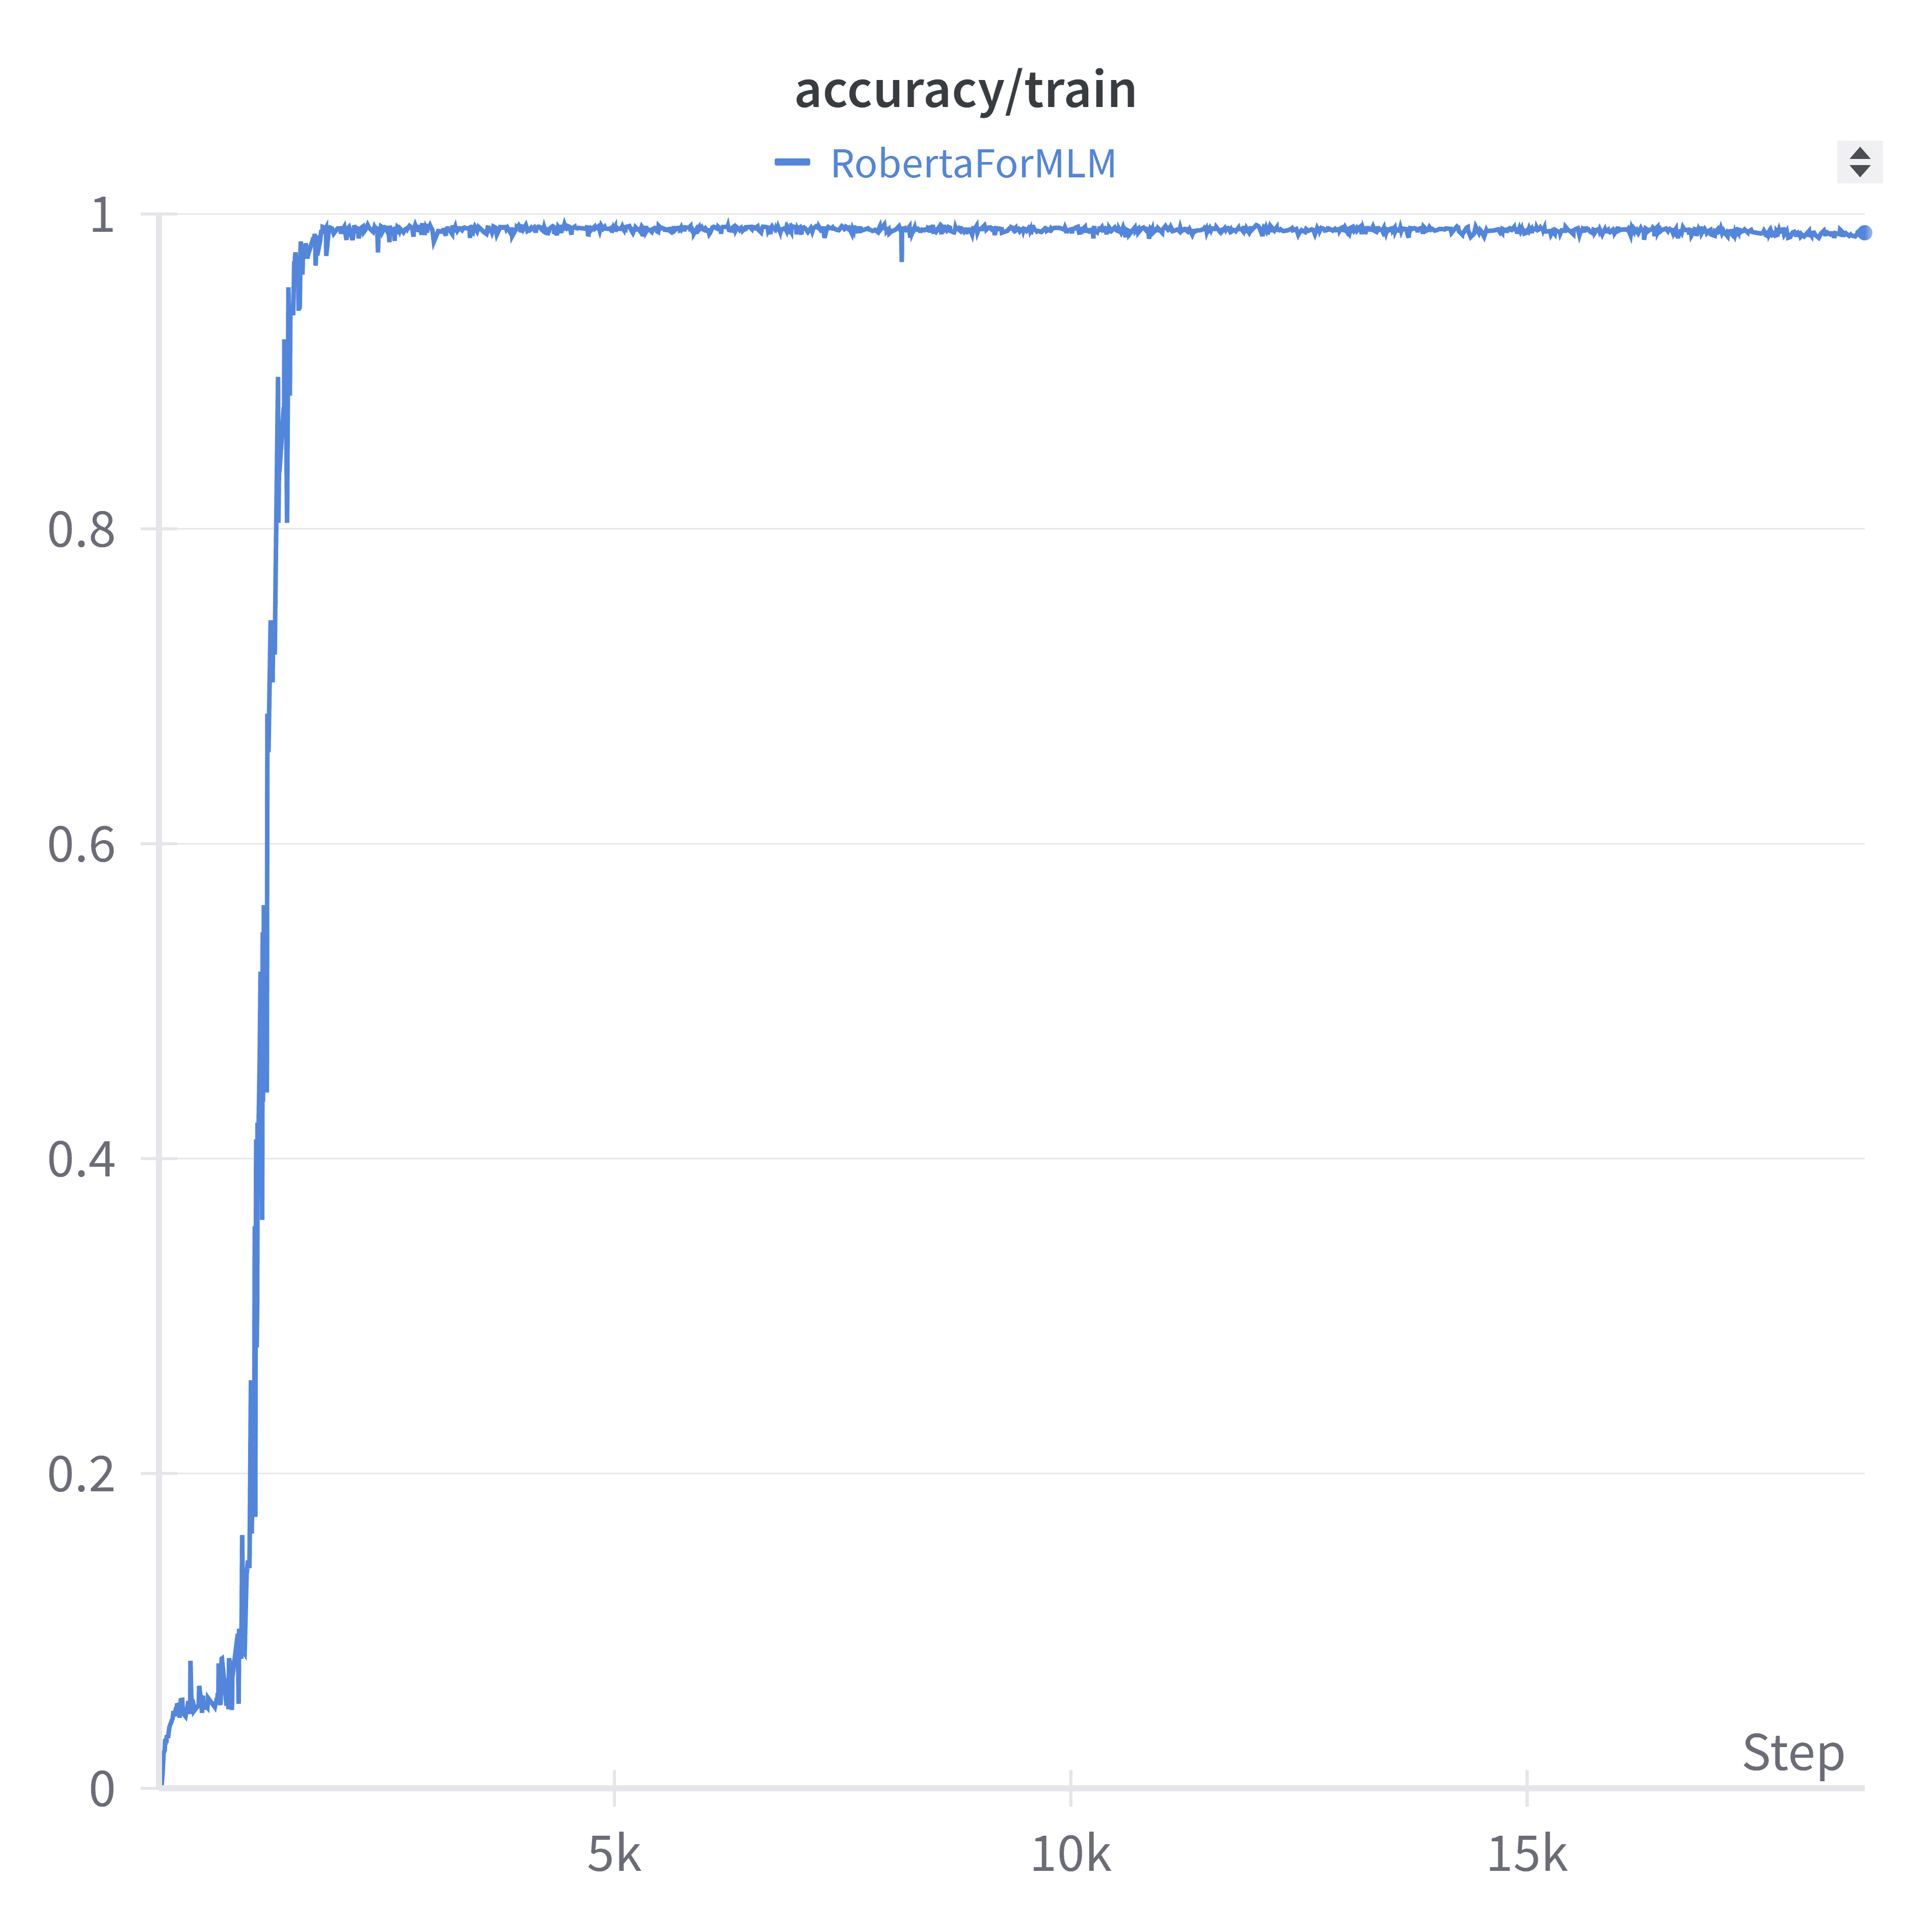
\includegraphics[width =  \textwidth ]{Bachelor-Thesis-Template/images/roberta/train/accuracy_train.png}
    \end{minipage}%
    \begin{minipage}{0.33\textwidth}
        \centering
        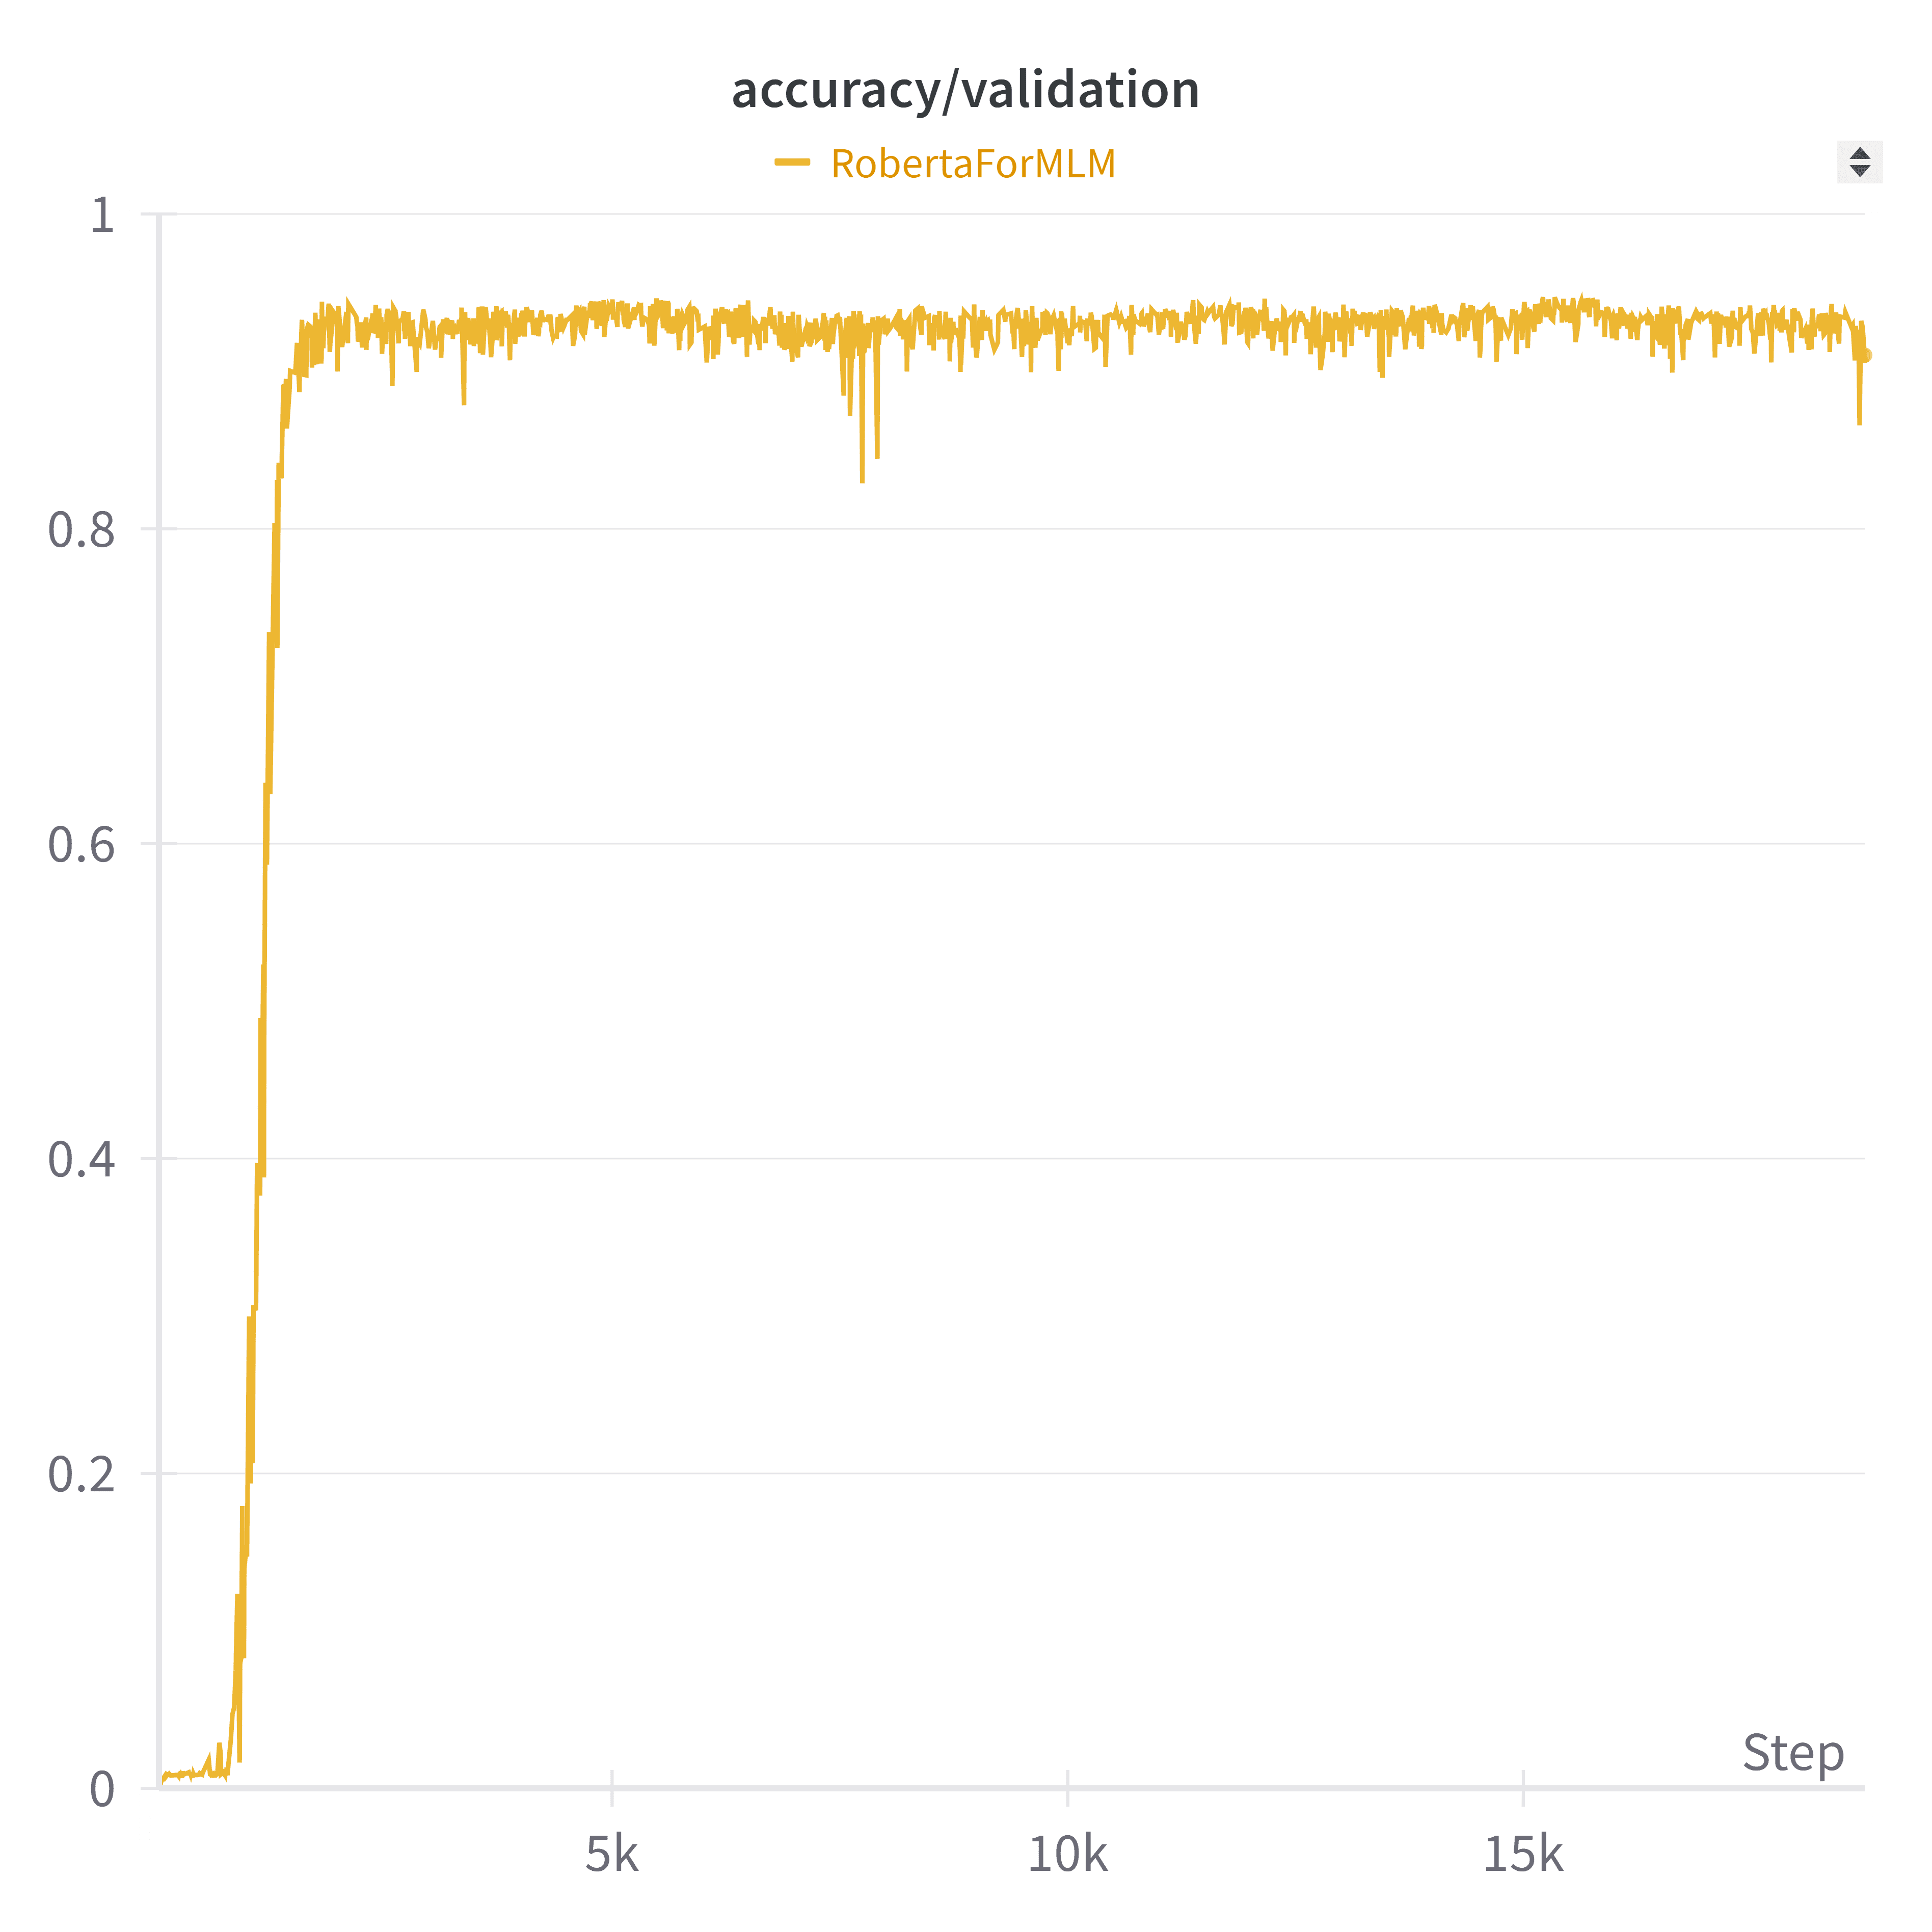
\includegraphics[width =  \textwidth ]{Bachelor-Thesis-Template/images/roberta/validation/accuracy_validation.png}
    \end{minipage}%
    \begin{minipage}{0.33\textwidth}
        \centering
        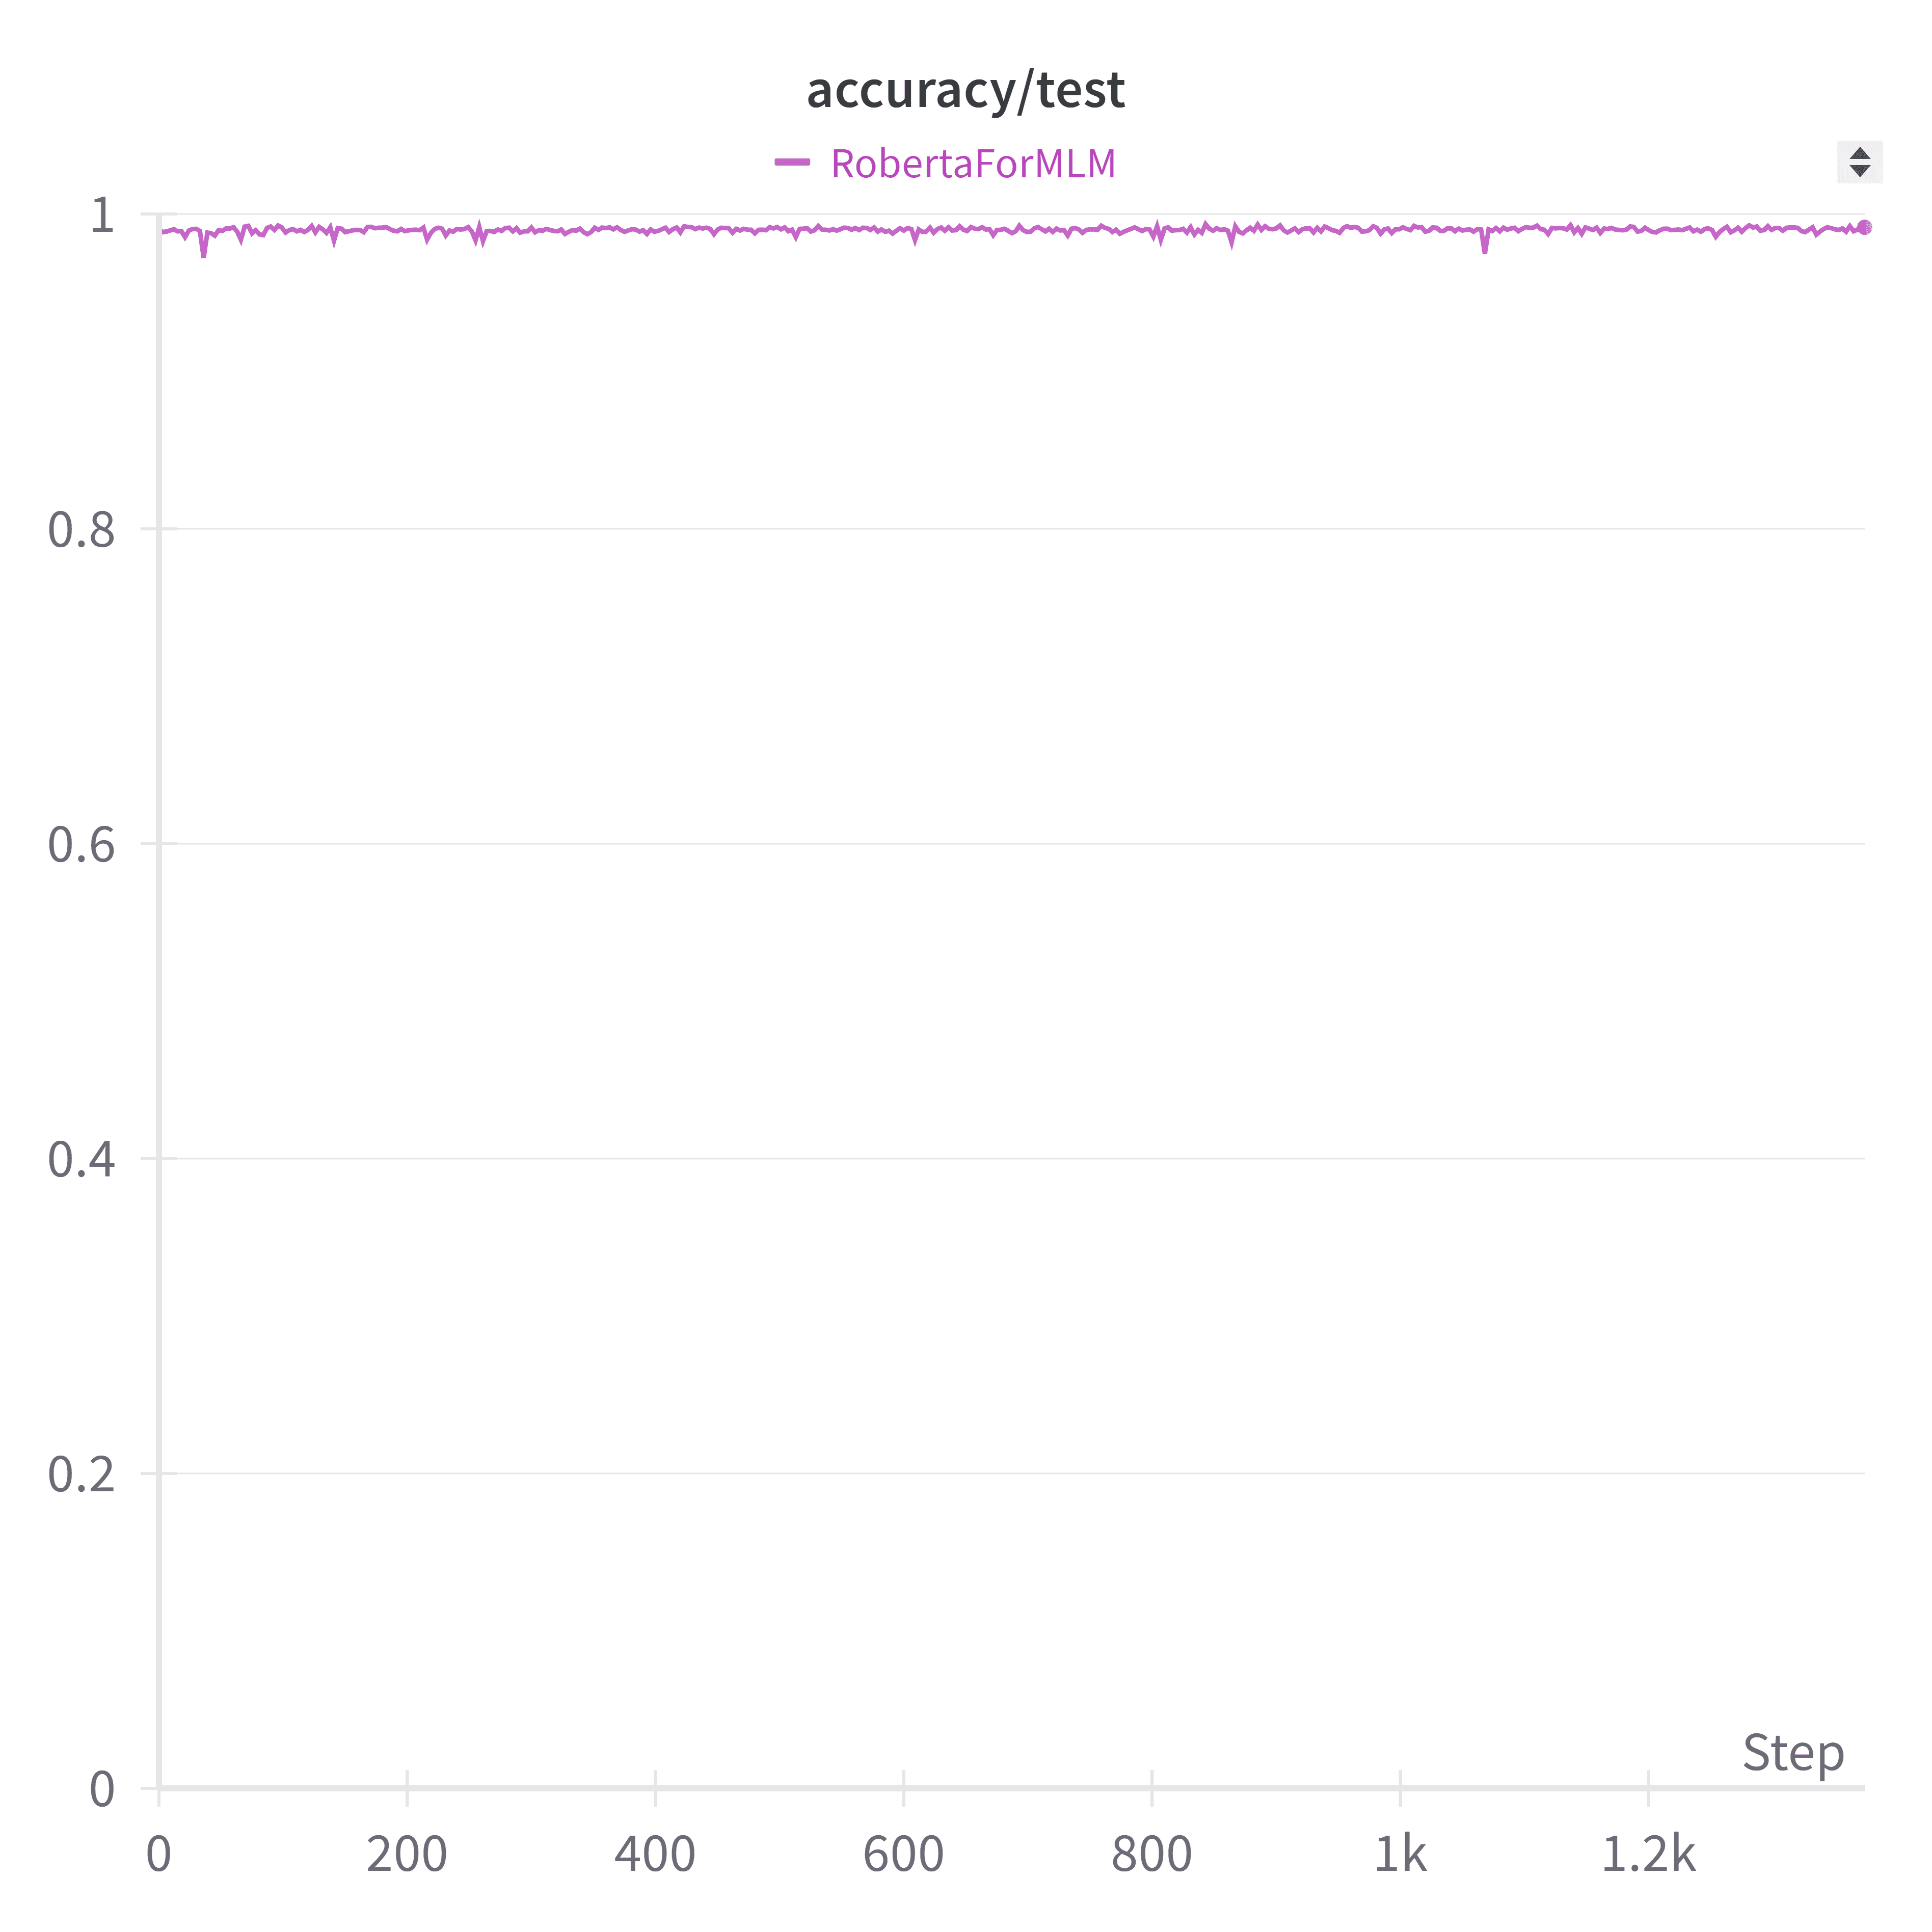
\includegraphics[width =  \textwidth ]{Bachelor-Thesis-Template/images/roberta/test/accuracy_test.png}
    \end{minipage}%

    \newline
    \begin{minipage}{0.33\textwidth}
      \centering
    \textbf{(a)}
    \end{minipage}%
    \begin{minipage}{0.33\textwidth}
    \centering
    \textbf{(b)}
    \end{minipage}%
    \begin{minipage}{0.33\textwidth}
    \centering
    \textbf{(c)}
    \end{minipage}%
    
    \caption{\small Графики метрики accuracy: (a) train, (b) validation, (c) test}
    \label{fig:roberta_accuracy}
\end{figure}

Результаты тестирования подтверждают высокую производительность модели RoBERTa в задаче предсказания молекулярных свойств, что делает её перпективным инструментом для дальнейших исследований в области хемоинформатики.

\subsection{Обучение MolCLR}
Процесс обучения включает следующие шаги:
\begin{enumerate}
\item В начале исследования был создан экземпляр \texttt{MoleculeDataset} на основе датасета ChemBL \cite{ChemBL}. Далее были определены индексы для обучающего, валидационного и тестового наборов данных. Для каждого из этих наборов данных был создан \texttt{DataLoader} из библиотеки \texttt{torch\_geometric} \cite{torch_geometric}, который использовался для итерации по данным в процессе обучения и валидации.

\item В качестве основы для обучения была выбрана самописная модель \texttt{MolecularGraph}. Эта модель включает в себя графовую модель (в зависимости от конфигурации это может быть \texttt{GINet} или \texttt{GCN}), а также линейный слой для предсказания. GNN была инициализирована с предварительно обученными весами.

\item В ходе обучения вычислялась функция потерь между предсказанными и истинными метками и выполнялось обратное распространение ошибки. В качестве метрики была выбрана L1-норма. Результатом одной эпохи было усреднение loss-функции по всей эпохе.

\newpage
\textbf{Код цикла обучения:}
\begin{lstlisting}
model = MolecularGraph().to(device)
loss_func = torch.nn.L1Loss()
def train_loop():
    train_tqdm = tqdm(train_dataloader, unit="batch")
    train_tqdm.set_description(f'Epoch {epoch_counter}')
    loss_sum = 0
    
    model.train()
    for (batch, labels_batch) in train_tqdm:
        optimizer.zero_grad()

        graph_batch = batch.to(device)
        labels_batch = labels_batch.to(device)

        predicted_labels = model(graph_batch)

        loss = loss_func(predicted_labels, labels_batch)
        loss.backward()

        loss_sum += loss.item()

        optimizer.step()
        train_tqdm.set_postfix(loss=loss.item())
    return loss_sum / len(train_dataloader)
\end{lstlisting}
\item В цикле валидации \texttt{eval\_loop()} был выполнен проход по каждому батчу в валидационном \texttt{eval\_dataloader}. Процесс был аналогичен циклу обучения, однако в этом случае веса модели не обновлялись. Валидация происходила каждую эпоху.

\item После каждой эпохи проводилось сравнение фукнции потерь на обучающем и валидационном наборах данных. Это позволило отслеживать процесс обучения и валидации модели в динамике.
\end{enumerate}


Данное обучение было проведено на 4 физических свойствах молекул: Polar Surface Area, AlogP, Bioactivities и Molecular Weight. В ходе эксперимента были получены следующие результаты. На рисунке \ref{fig:molclr_loss} представлены графики функции потерь в процессе обучения (a) и валидации (b) для этих четырех свойств.

На тестовой выборке были получены следующие значения функции потерь:

\begin{itemize}
\item Molecular Weight: 99.521
\item Polar Surface Area: 20.127
\item AlogP: 1.019
\item Bioactivities: 5.74
\end{itemize}

В данном датасете свойство Molecular Weight лежит в пределах [77.06; 1060.97] со средним 388.6, свойство Polar Surface Area лежит в пределах [0.0; 392.73] со средним 78.5. свойство AlogP лежит в пределах [-5.61; 11.97] со средним 3.33, свойство Bioactivities лежит в пределах [1.0; 3247.0] со средним 12.1. Эти данные показывают, что диапазоны и средние значения для каждого из четырех свойств существенно различаются. Поэтому, чтобы сравнить производительность модели на разных свойствах, необходимо рассмотреть относительные значения функции потерь:
\begin{itemize}
\item Molecular Weight: $99.521 / 388.6 = 0.26$
\item Polar Surface Area: $20.127 / 78.5 = 0.26$
\item AlogP: $1.019 / 3.33 = 0.31$
\item Bioactivities: $5.74 / 12.1 = 0.47$
\end{itemize}

Эти результаты указывают на то, что модель наиболее точно предсказывает свойства Molecular Weight и Polar Surface Area, в то время как для свойства Bioactivities значение функции потерь значительно выше, что может указывать на необходимость дальнейшей оптимизации модели для этого свойства.

\begin{figure}[h]
    \begin{minipage}{0.5\textwidth}
        \centering
        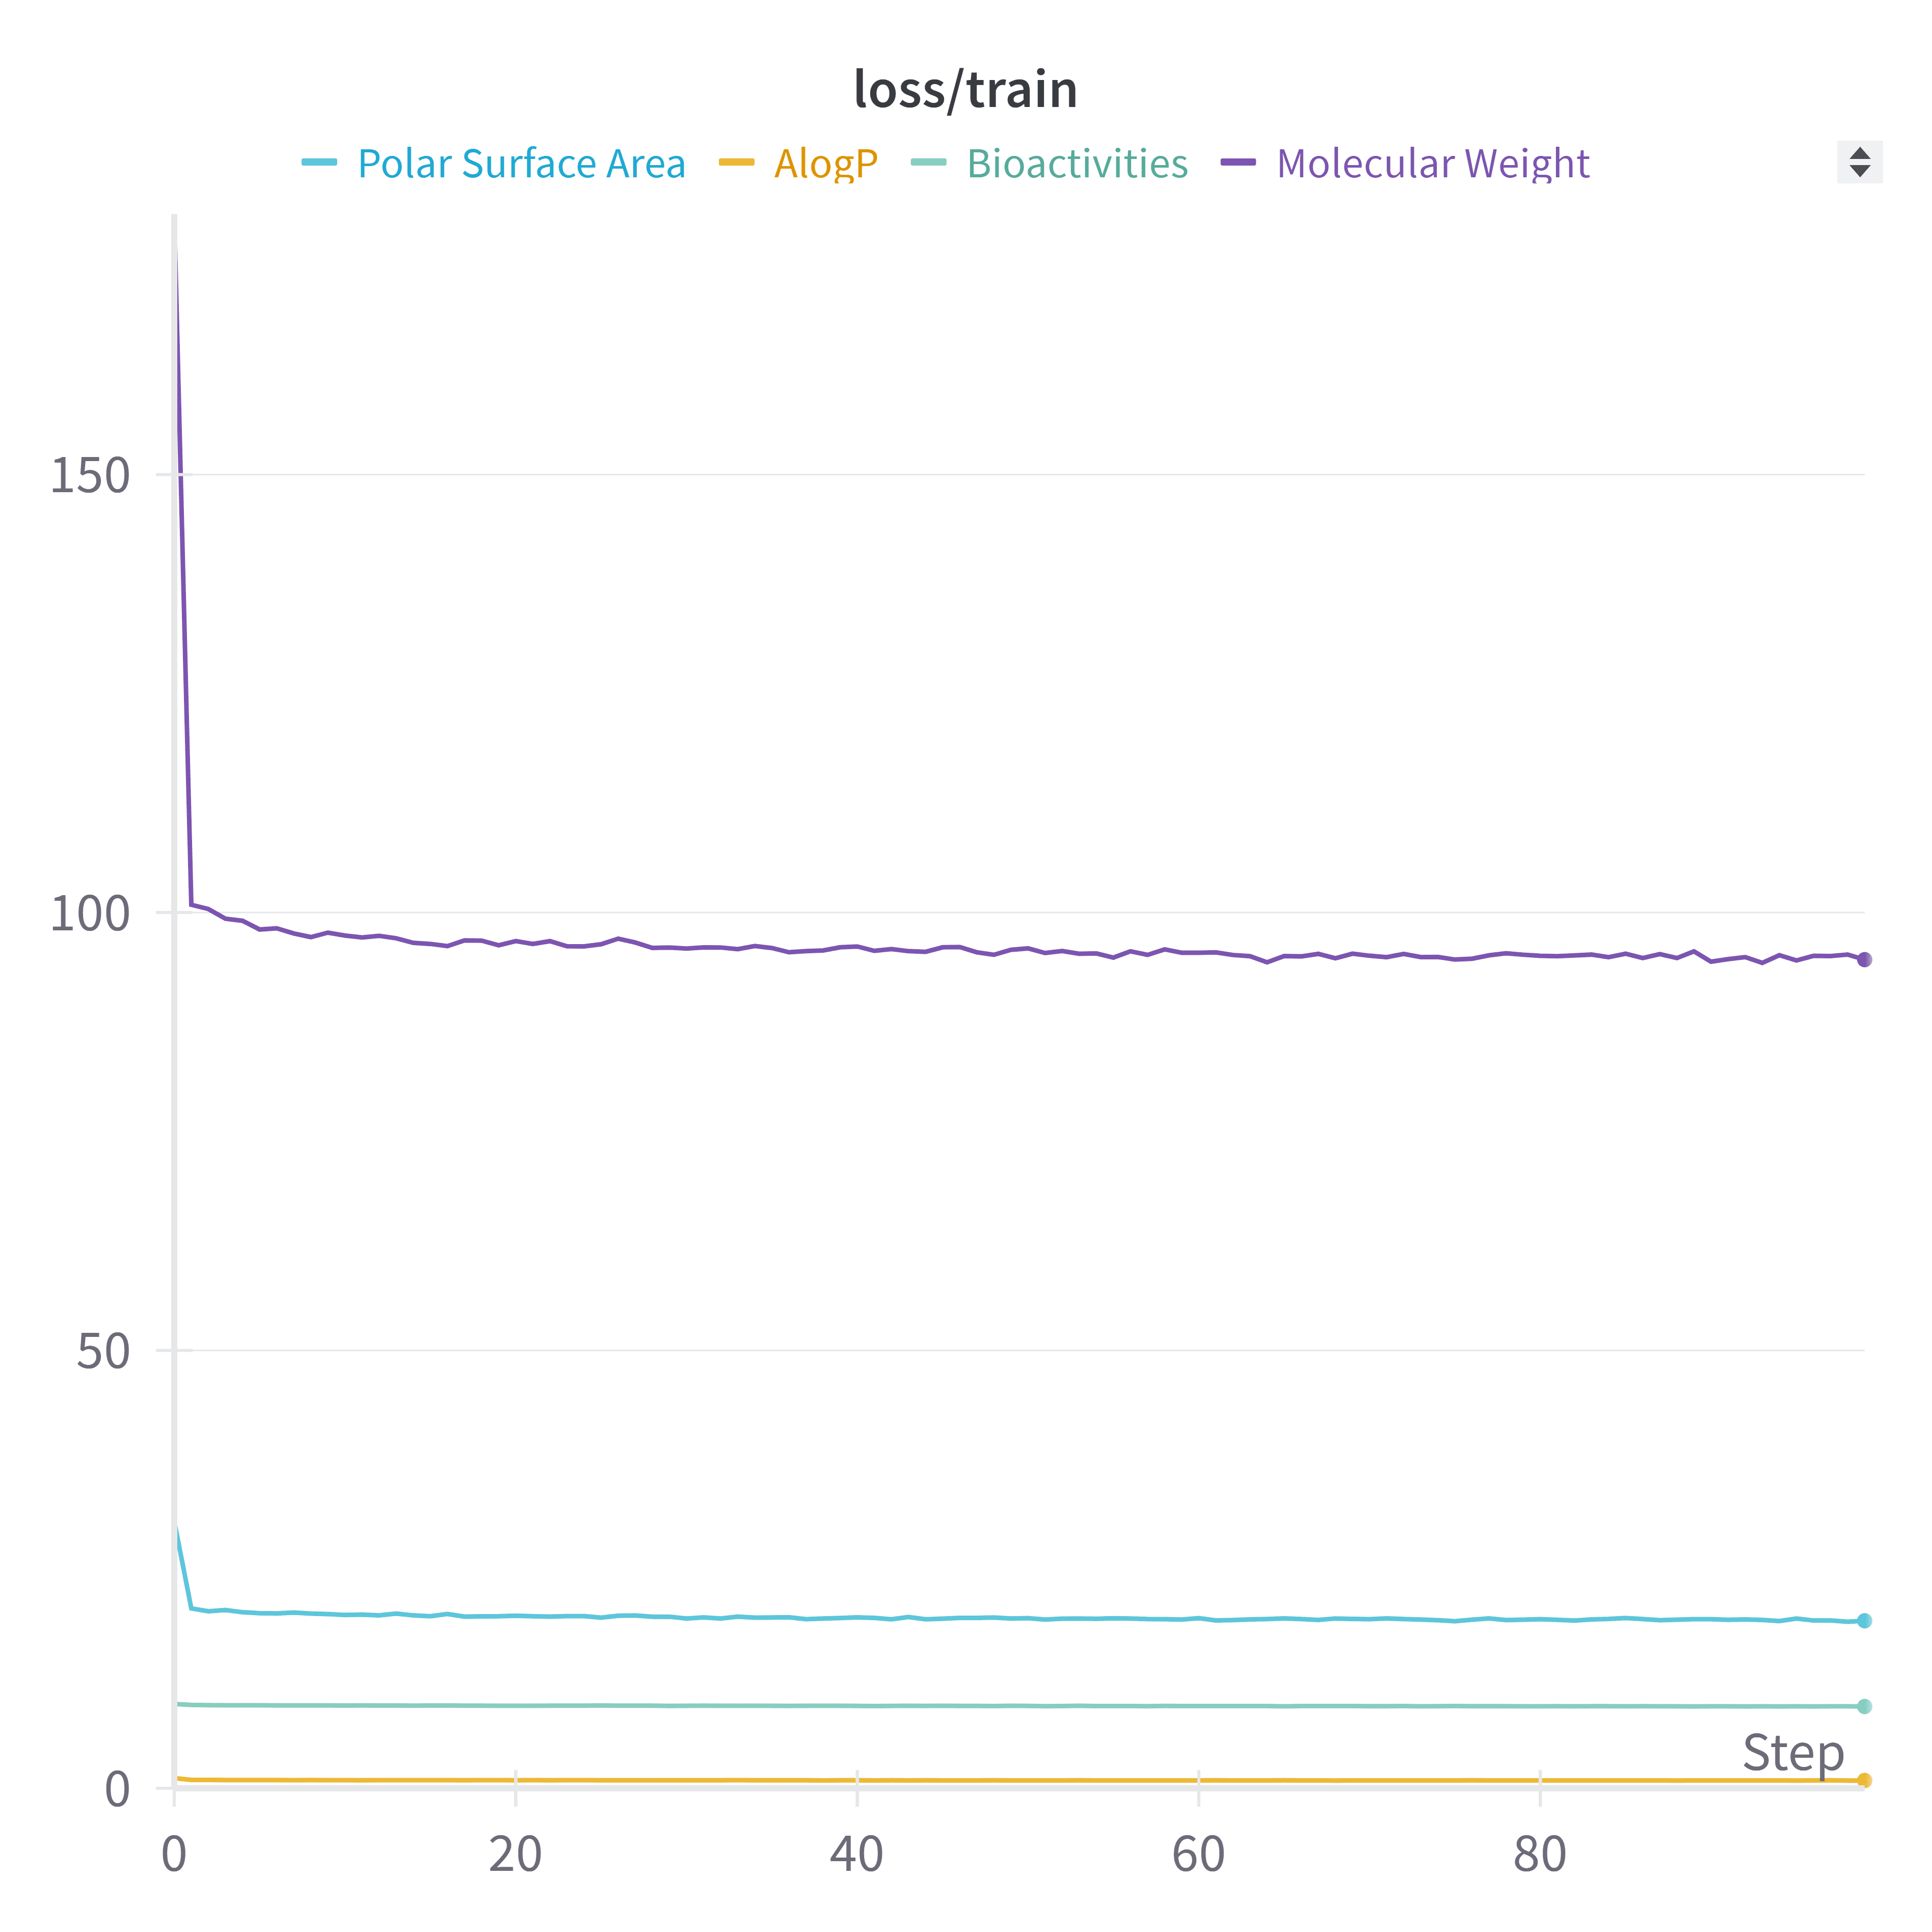
\includegraphics[width =  \textwidth ]{Bachelor-Thesis-Template/images/molclr/MolCLR loss_train.png}
    \end{minipage}%
    \begin{minipage}{0.5\textwidth}
        \centering
        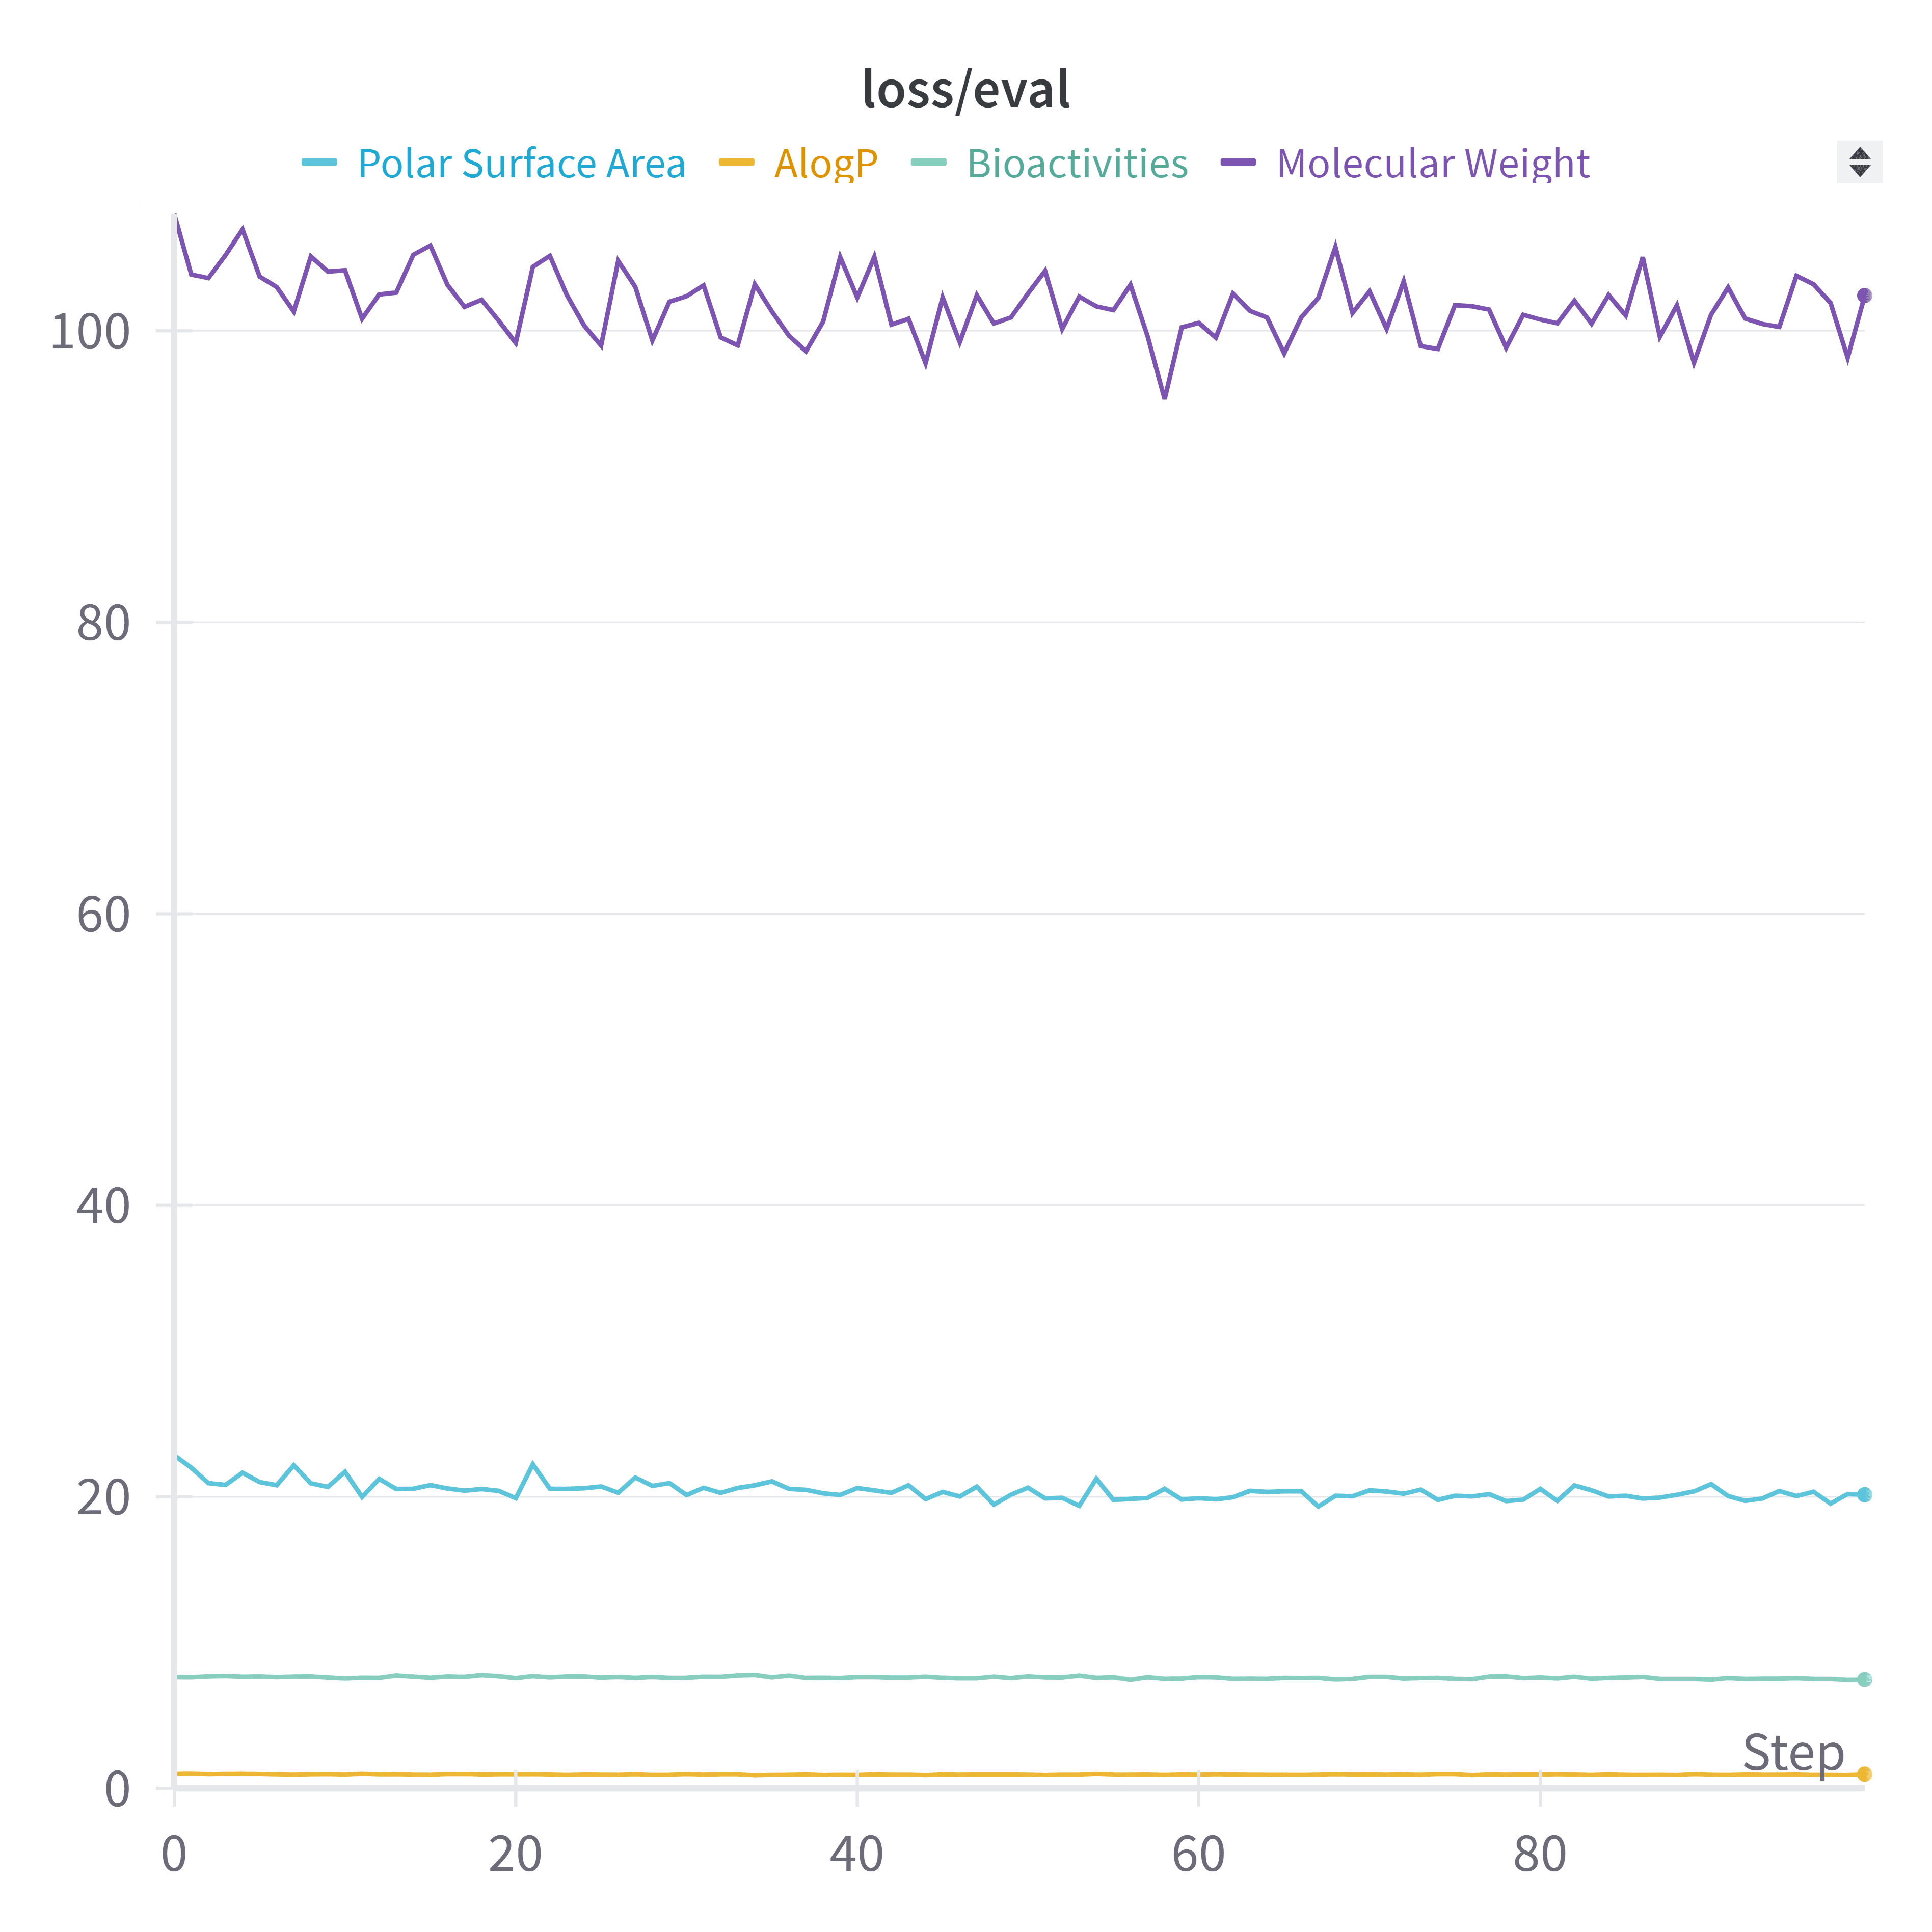
\includegraphics[width =  \textwidth ]{Bachelor-Thesis-Template/images/molclr/MolCLR loss_eval.png}
    \end{minipage}%

    \newline
    \begin{minipage}{0.5\textwidth}
      \centering
    \textbf{(a)}
    \end{minipage}%
    \begin{minipage}{0.5\textwidth}
    \centering
    \textbf{(b)}
    \end{minipage}%
    
    \caption{\small Графики функции потерь L1-loss: (a) train, (b) validation}
    \label{fig:molclr_loss}
\end{figure}
% Molecular Weight mean is 388.62499576450654
% Molecular Weight max is 1060.97
% Molecular Weight min is 77.06
% Bioactivities mean is 12.074121135112241
% Bioactivities max is 3247.0
% Bioactivities min is 1.0
% AlogP mean is 3.337519059720458
% AlogP max is 11.97
% AlogP min is -5.61
% Polar Surface Area mean is 78.52042037272342
% Polar Surface Area max is 392.73
% Polar Surface Area min is 0.0

\subsection{Обучение Graphormer}
Обучение Graphormer включает в себя использование специализированных слоёв внимания, которые позволяют модели учитывать глобальные структурные особенности графа. Этап обучения направлен на минимизацию функции потерь и оптимизацию параметров модели для достижения наилучшей производительности. В данном эксперименте используется функция потерь MSE (Mean Squared Error). Для оптимизации параметров применяется классический оптимизатор AdamW с коэффициентом обучения равным 5e-5. Кроме того, используется линейный планировщик скорости обучения.

\newcommand\wtt[1]{%
  \hfil\penalty0\hfilneg\texttt{#1}%
}

\begin{enumerate}
\item Сначала из части датасета ChemBL \cite{ChemBL} инстанцируется экземпляр класса \texttt{Dataset} библиотеки HuggingFace \cite{huggingface}. Далее идет разделение всего набора данных на обучающий, валидационный и тестовый наборы. Это дает 80\% данных для обучения, 10\% для валидации и 10\% для тестирования.

\item Затем применяется специальная функция \texttt{preprocess\_item} к каждому элементу в наборах данных. Это преобразует каждый элемент в формат, подходящий для модели Graphormer (добавляются еще 7 тензоров для каждой молекулы).

\item Инициализируется модель \texttt{GraphormerForGraphClassification} (использовался чек-поинт \texttt{clefourrier/graphormer-base-pcqm4mv1}). Также устанавливается параметр \texttt{num\_classes} равным 1, поскольку предсказывается одно свойство.

\item Инициализируется GraphormerDataCollator, который позволяет обьединять данные графов в батчи (в отличие от обычных GNN, где \texttt{torch\_geometric.data} обьекты графов подаются на вход по одному). Данный обраточик данных подается в инициализацию Dataloaders для каждого набора данных.

\item Инициализируется \textbf{оптимизаторы обучения:}
\begin{lstlisting}
from transformers import AdamW, get_scheduler

num_epoch = 100
num_training_steps = num_epoch * len(train_dataloader)

optimizer = AdamW(model.parameters(), lr=5e-5)
lr_scheduler = get_scheduler(
    'linear',
    optimizer = optimizer,
    num_warmup_steps = 5,
    num_training_steps = num_training_steps,
)
\end{lstlisting}


\item Далее исполняется стандартный \textbf{цикл обучения:}
\begin{lstlisting}
progress_bar_train = tqdm(range(num_training_steps))

model.train()
train_epoch_loss = 0
for batch in train_dataloader:
    input_batch = { k: v.to(device) for k, v in batch.items() }
    
    outputs = model(**input_batch)
    
    loss = outputs["loss"]
    loss.backward()
    train_epoch_loss += loss.item()
    
    optimizer.step()
    lr_scheduler.step()
    optimizer.zero_grad()
    progress_bar_train.update(1)
\end{lstlisting}

\item В цикле валидации итерация проходт по каждому батчу в \texttt{eval\_dataloader}. Процесс похож на цикл обучения, но здесь не обновляются веса модели.

\item После каждой эпохи сравниваются функции потерь на обучающем и валидационном наборах данных. Эти данные сохраняются с помощью  библиотеки wandb \cite{wandb}. С помощью одноименного веб-сервиса можно будет отследить, как модель обучалась и валидировалась в процессе обучения.
\end{enumerate}

Результаты работы данного алгоритма показаны на рисунке \ref{fig:graphormer_vs_molclr_loss}. На рисунке (a) изображен график обучения Graphormer с помощью регресии молекулярного свойсва Molecular Weight. Также здесь представлен график обучения модели MolCLR для сравнения результатов. Рядом, на рисунке (b), показаны результаты валидации этих двух моделей. Исходя из этих данных, понятно, что трансформер Graphormer имеет потенциал предсказывания молекулярных свойств выше, чем модель MolCLR, основанная на классической модели свертки графов. Поэтому исследуемый Graphormer может быть использован как альтернатива или дополнение к модели MolCLR.


В ходе исследования была предпринята попытка нормализации данных с использованием MinMaxScaler из библиотеки sklearn \cite{sklearn}. Однако, после нормализации данные оказывались слишком близкими к нулю, что приводило к погрешностям в вычислениях и делало графики менее информативными. В связи с этим, результаты исследования показаны с использованием исходных, ненормализованных данных для обучения модели Graphormer.



\begin{figure}[h]
    \begin{minipage}{0.5\textwidth}
        \centering
        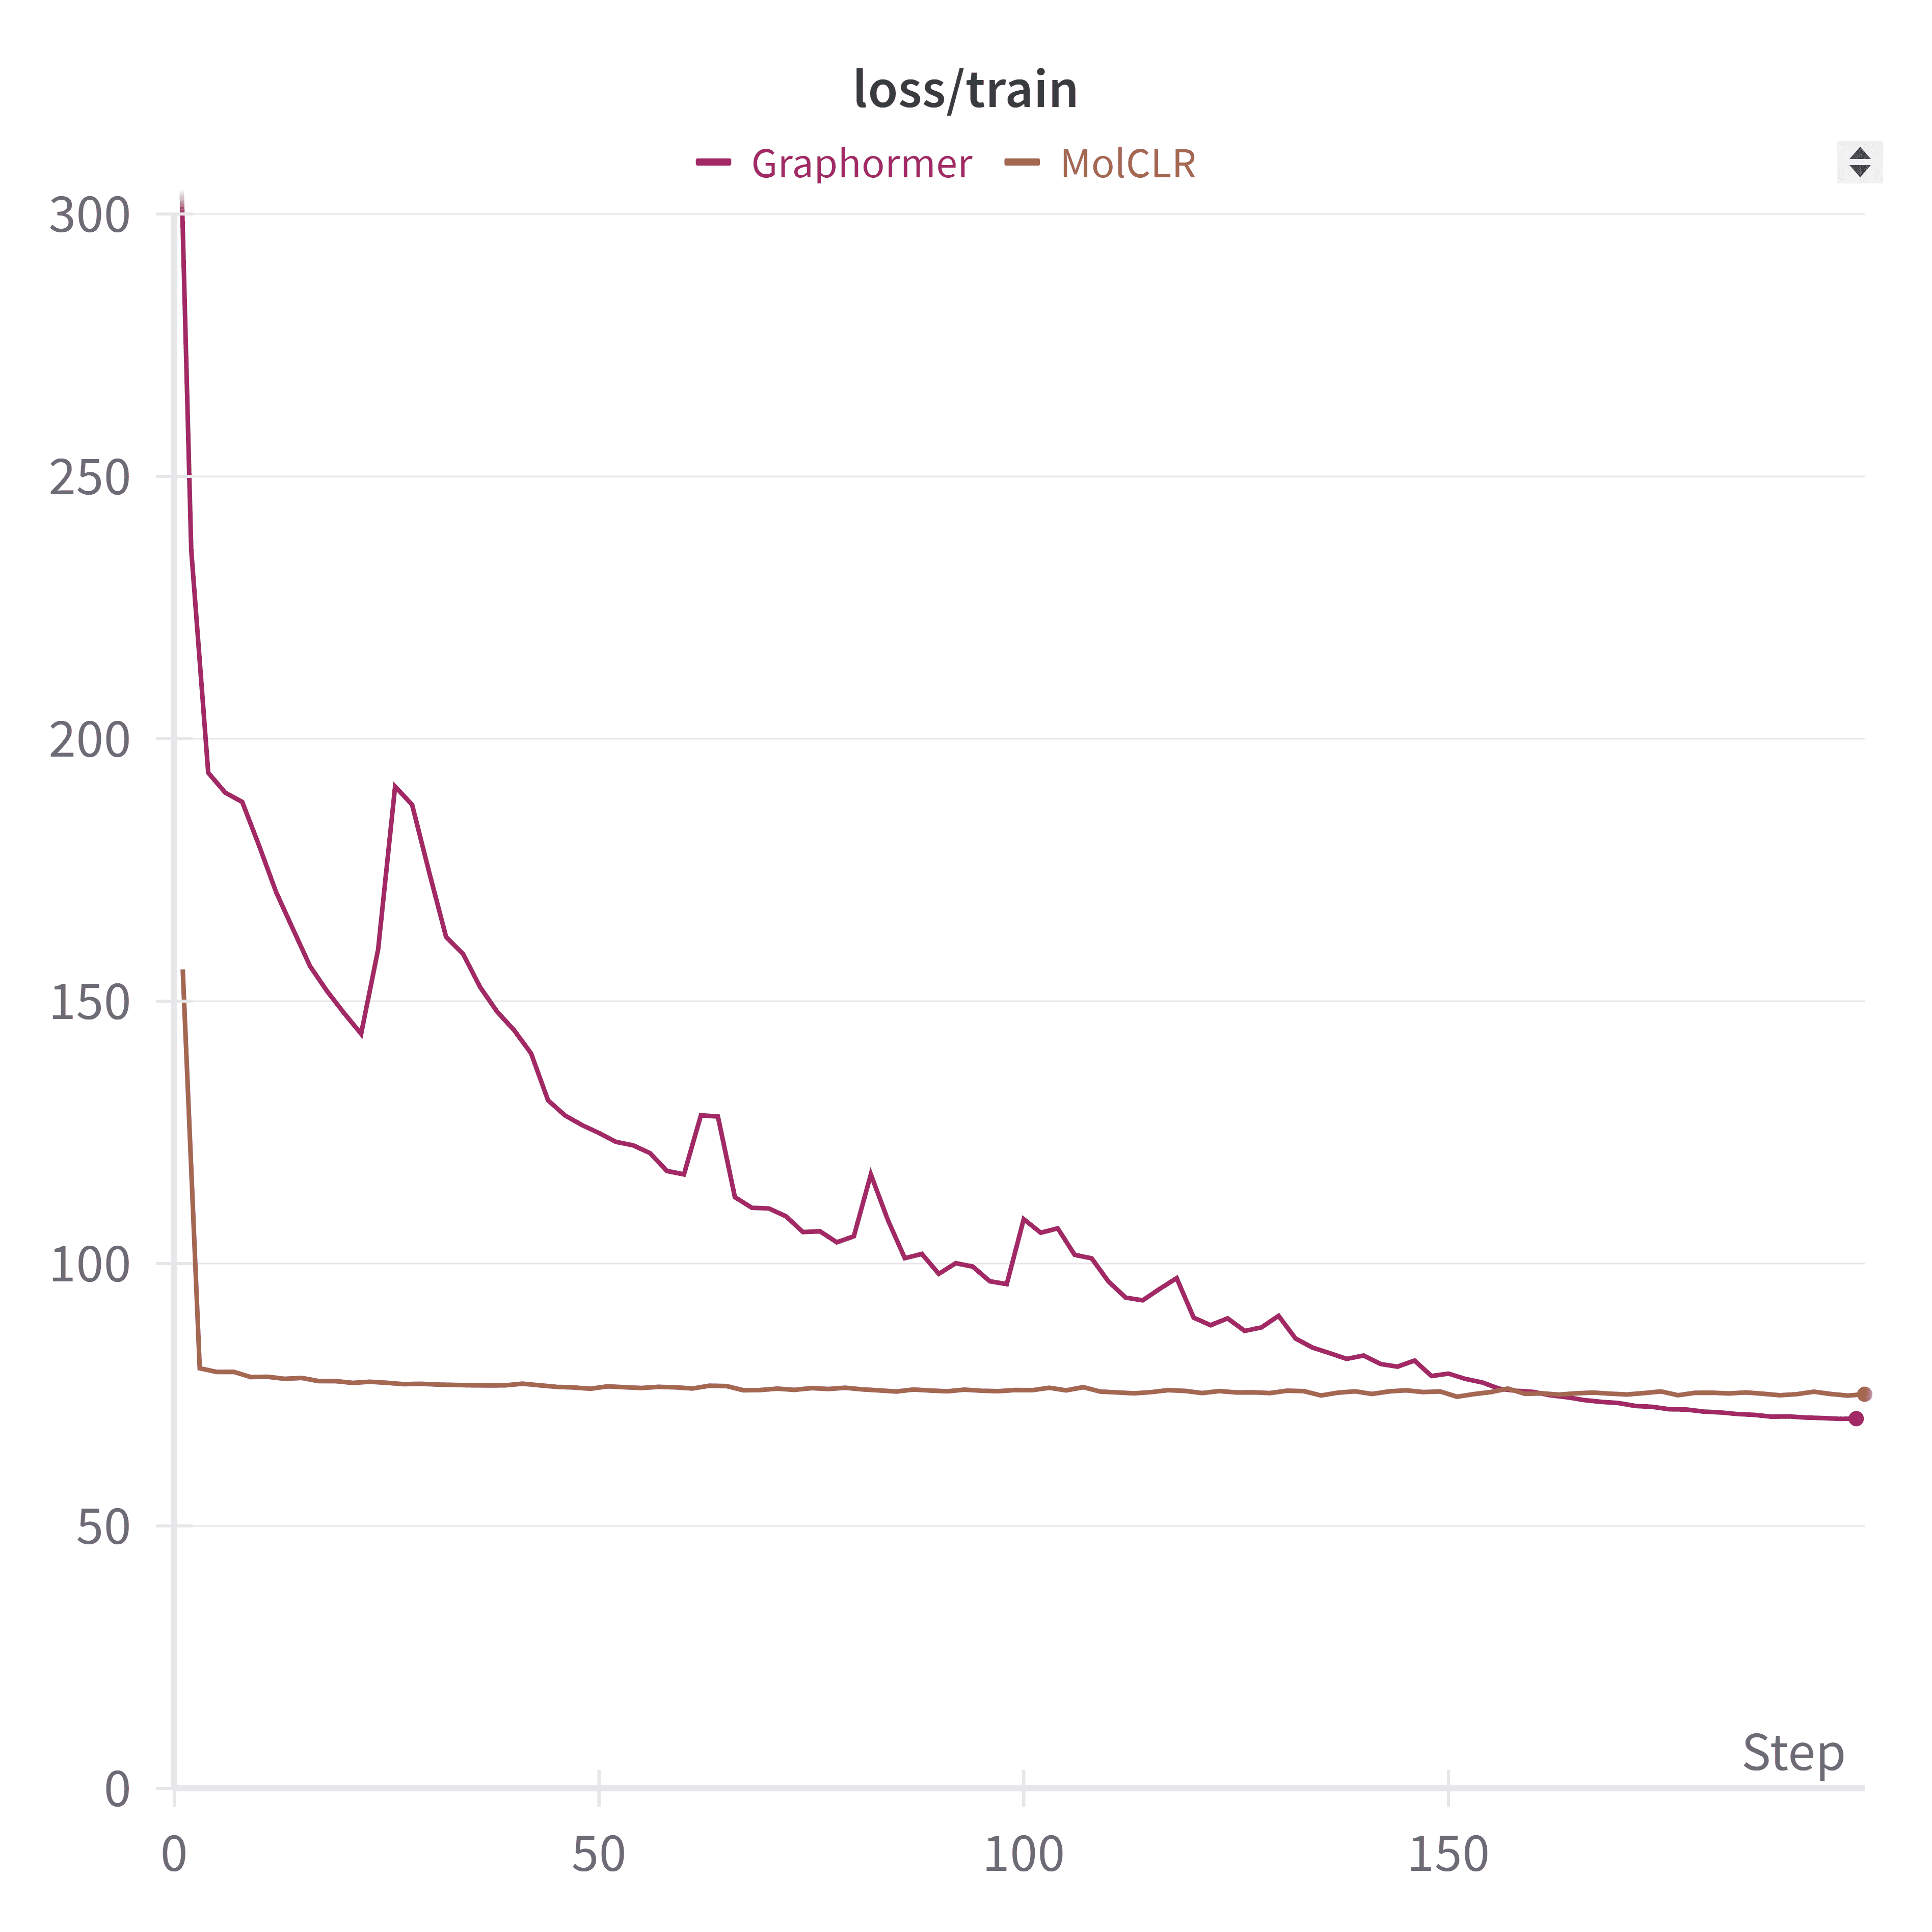
\includegraphics[width =  \textwidth ]{Bachelor-Thesis-Template/images/graphormer/train_graphormer.png}
    \end{minipage}%
    \begin{minipage}{0.5\textwidth}
        \centering
        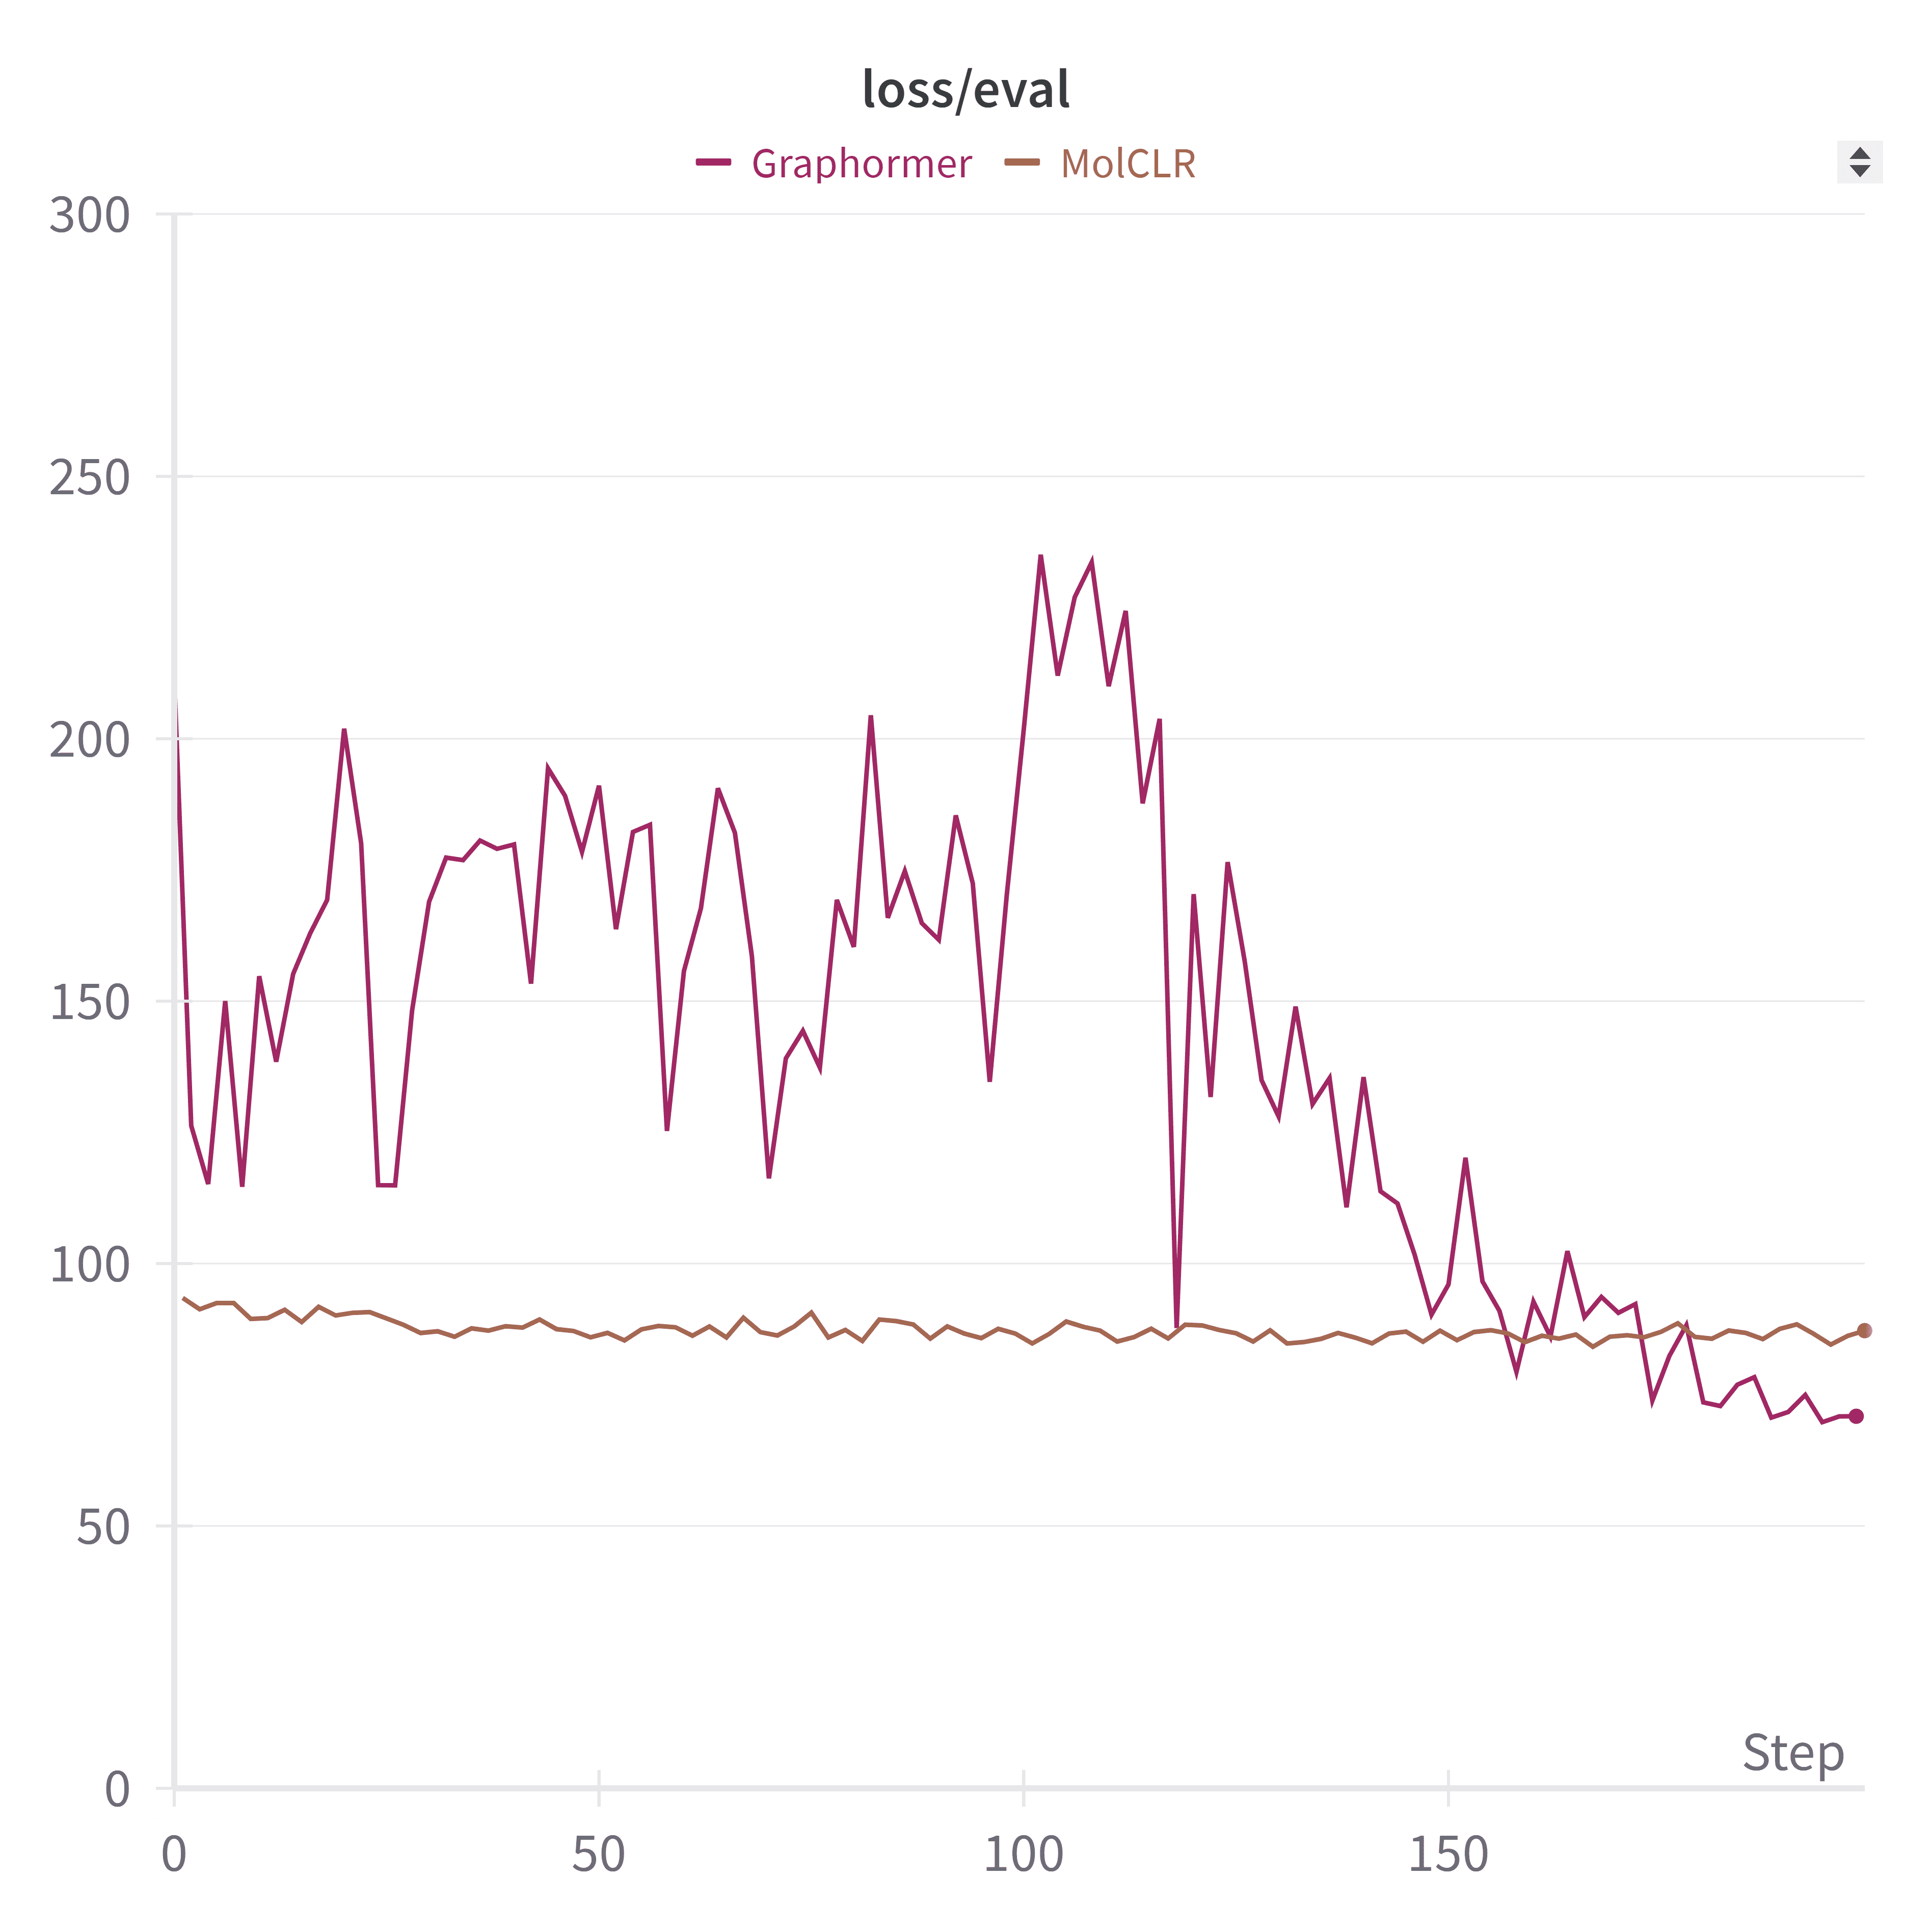
\includegraphics[width =  \textwidth ]{Bachelor-Thesis-Template/images/graphormer/eval_graphormer.png}
    \end{minipage}%

    \newline
    \begin{minipage}{0.5\textwidth}
      \centering
    \textbf{(a)}
    \end{minipage}%
    \begin{minipage}{0.5\textwidth}
    \centering
    \textbf{(b)}
    \end{minipage}%
    
    \caption{\small Сравнение графиков функций потерь Graphormer и MolCLR: (a) train, (b) validation}
    \label{fig:graphormer_vs_molclr_loss}
\end{figure}

\subsection{Разработка и реализация baseline-модели}
В данном разделе будет рассмотрен подход к обучению двух моделей на основе разных представлений молекулярных данных. В качестве отправной точки, или “бейзлайна”, были выбраны две модели: RoBERTa \cite{liu2019roberta} и MolCLR \cite{molclr}. Эти модели были выбраны из-за их эффективности в обработке текстовых и графовых данных соответственно, а также из-за относительной простоты их объединения. Для приближения эмбеддингов, полученных от каждой из этих моделей, использовалась функция косинусоидальной близости CosineSimilarityLoss. Обучение проводилось на датасете ChemBL. \cite{ChemBL}
Общая схема модели изображена на рисунке \ref{fig:bert_plus_molclr}.

\begin{figure}[h]
    \centering
    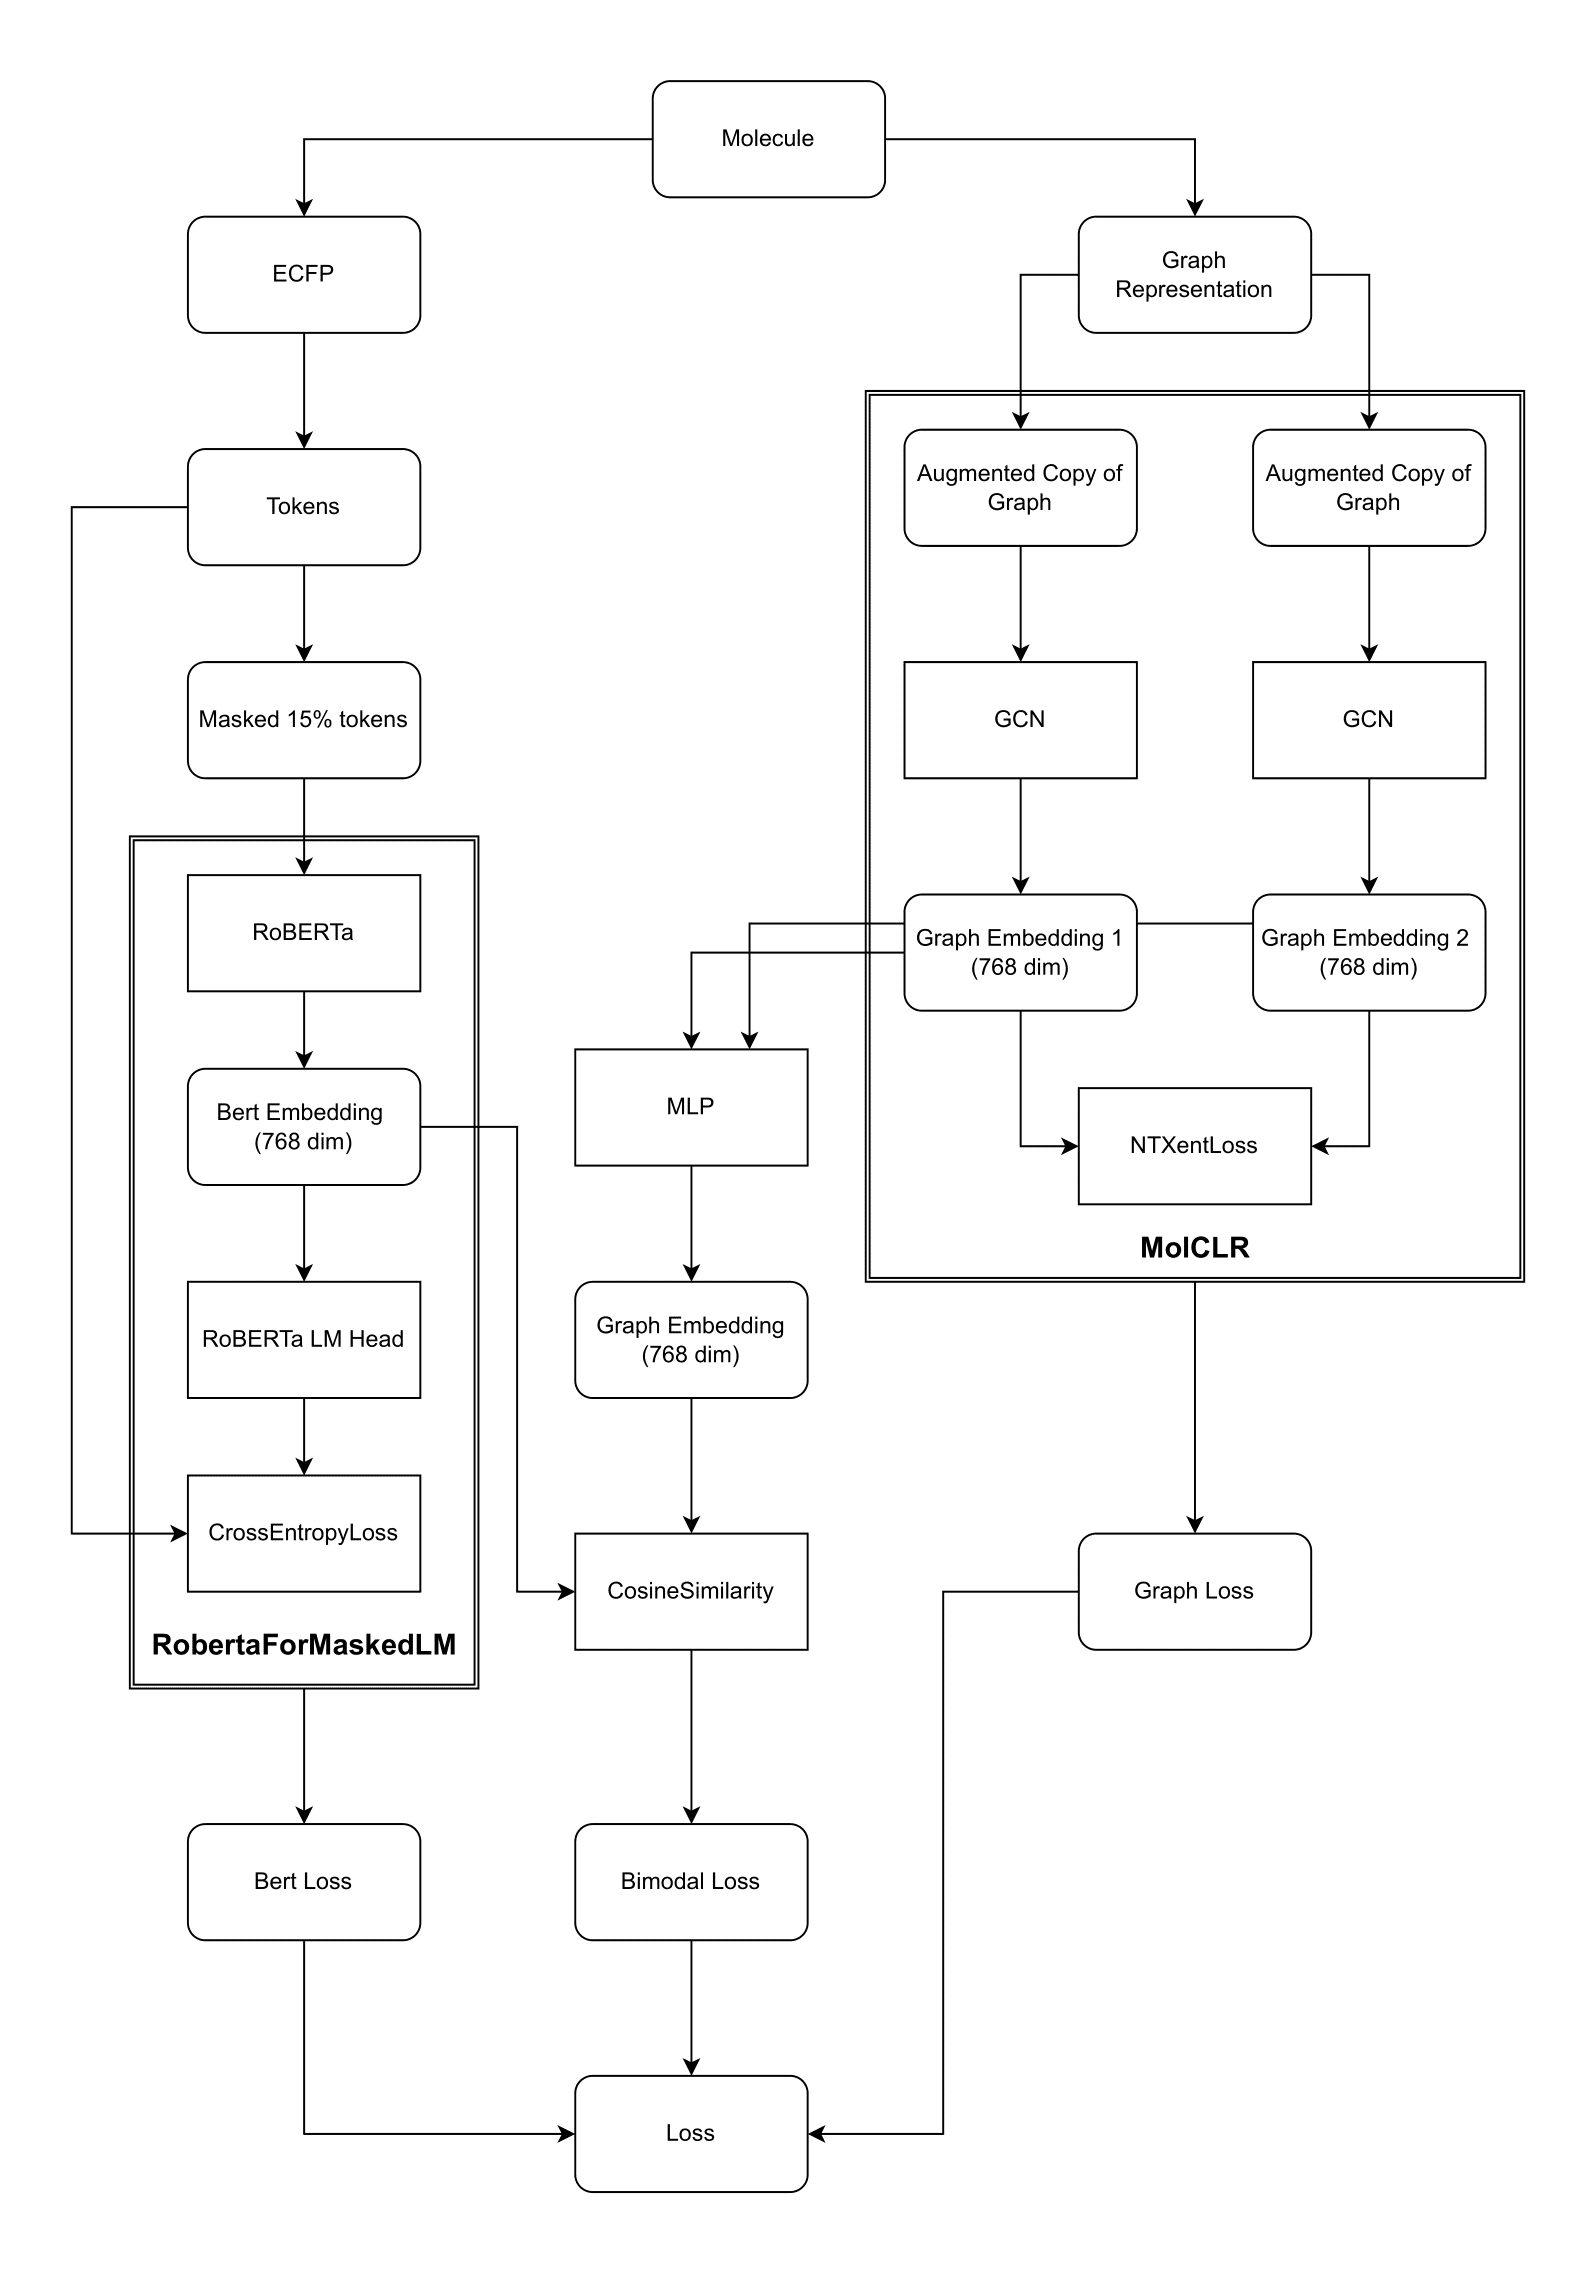
\includegraphics[width = 0.7 \textwidth ]{Bachelor-Thesis-Template/images/scheme.png}
    
    \caption{\small Архитектура объединения двух моделей RoBERTa и MolCLR.}
    \label{fig:bert_plus_molclr}
\end{figure}

\subsubsection{Описание алгоритма обучения}
\begin{enumerate}
    \item Инициализация класса MoleculeDataset, который наследуется от класса Dataset из библиотеки \texttt{torch\_geometric} и предназначен для создания набора данных из молекулярных структур, представленных в формате SMILES. Полученный набор данных состоит из токенов для входа модели трансформера, а также двух графовых представлений одной молекулы, которое используется в MoLCLR. Токены получаются применением вышеопределенных функций \texttt{tokenize} и \texttt{mlm}. Графовые представления являются агментированными копиями графа молекулы. 
    Метод класса MoleculeDataset \texttt{\_\_getitem\_\_}:
    \begin{lstlisting}
def __getitem__(self, index):
    node_feat, edge_index, edge_attr, num_nodes, num_edges = self.get_graph_from_smiles(self.dataset['Smiles'][index])

    graph_i = self.get_augmented_graph_copy(node_feat, edge_index, edge_attr, num_nodes, num_edges)
    graph_j = self.get_augmented_graph_copy(node_feat, edge_index, edge_attr, num_nodes, num_edges)

    ecfp = self.dataset['ecfp1'][index]
    data_for_bert = self.apply_mlm(self.tokenize(ecfp))
    return data_for_bert, graph_i, graph_j
    \end{lstlisting}
    \item Инициализация класса MolecularBertGraph: Этот класс представляет собой модель, которая объединяет модель \texttt{RobertaForMaskedLM} и графовую нейронную сеть MolCLR:
    \begin{lstlisting}
from transformers import RobertaForMaskedLM
from transformers import RobertaConfig

if config['model_type'] == 'gin':
    from MolCLR.models.ginet_molclr import GINet as GraphModel
elif config['model_type'] == 'gcn':
    from MolCLR.models.gcn_molclr import GCN as GraphModel
else:
    raise ValueError('GNN model is not defined in config.')
from MolCLR.utils.nt_xent import NTXentLoss

class MolecularBertGraph(torch.nn.Module):
    def __init__(self):
        super(MolecularBertGraph, self).__init__()
        self.bert = RobertaForMaskedLM(roberta_config)
        self.graph_model = GraphModel(**config['model'])
        self.out_graph_linear = torch.nn.Linear(768 * 2, 768, bias=True)
        # contrastive loss for MolCLR
        self.nt_xent_criterion = NTXentLoss(self.batch_size, **config['loss'])
        # cosine distance as loss between models
        self.cosine_sim = torch.nn.CosineSimilarity(dim=-1)

    def forward(self, bert_batch, graph_batch1, graph_batch2):
        bert_output = self.bert(bert_batch)
        bert_loss = bert_output.loss
        bert_emb = bert_output.hidden_states[0][:, 0, :] # CLS embedding 

        graph_loss, hidden_states_1, hidden_states_2 = self.graph_step(graph_batch1, graph_batch2)
        graph_emb = self.out_graph_linear(torch.cat((hidden_states_1, hidden_states_2), dim=-1))

        bimodal_loss = ((1 - self.cosine_sim(bert_emb, graph_emb))**2).mean()
        return bert_loss, graph_loss, bimodal_loss

    def graph_step(self, xis, xjs):
        ris, zis = self.graph_model(xis)
        rjs, zjs = self.graph_model(xjs)
        # normalize projection feature vectors
        zis = torch.nn.functional.normalize(zis, dim=1)
        zjs = torch.nn.functional.normalize(zjs, dim=1)
        
        loss = self.nt_xent_criterion(zis, zjs)
        return loss, ris, rjs
    \end{lstlisting}
    \item Cоздание экземпляра MoleculeDataset, загрузчиков данных для обучающего и валидационного наборов данных, а также экземпляра MolecularBertGraph.
    \item Инициализация стандартного оптимизиматора AdamW с lr равным 5e-3.
    \item В цикле обучения вычисляется значения функции потерь \texttt{bert\_loss}, \texttt{graph\_loss}, \texttt{bimodal\_loss} на каждом батче из \texttt{train\_dataloader}. Финальное значение функции потерь вычисляется по формуле 
    
    $$\texttt{loss} = \alpha * \texttt{bert\_loss} + \beta * \texttt{graph\_loss} + \gamma * \texttt{bimodal\_loss}$$ 
    
    где $\alpha$, $\beta$, $\gamma$ - соответсвующие коэффиценты (гиперпараметры). Далее происходит обратное распространение ошибки. Результатом одной эпохи было усреднение всех значений функции потерь по всей эпохе.

    \item В цикле валидации \texttt{eval\_loop()} был выполнен проход по каждому батчу в валидационном \texttt{eval\_dataloader}. Процесс был аналогичен циклу обучения, однако в этом случае веса модели не обновлялись. Валидация происходила каждую эпоху.
    
    \item Далее идет основной цикл обучения, который выполняет заданное количество эпох обучения. В каждой эпохе выполняются обучающий и валидационный циклы, а также обновляются логи и сохраняются веса модели.

\end{enumerate}
В следующем разделе представлены графики обучения и валидации для всех четырех функций потерь: \texttt{bert\_loss}, \texttt{graph\_loss}, \texttt{bimodal\_loss} и \texttt{loss}. Эти графики помогут лучше понять динамику обучения и валидации модели, а также влияние каждой из компонент потери на общую функцию потерь.

\subsubsection{Результаты baseline-эксперимента}
Baseline эксперимент был проведен с двумя вариантами графовых моделей: GCN и GIN.
На рисунке \ref{fig:loss_bimodal} представлен график динамики общей функции потерь для двух моделей: RobertaForMaskedLM + MolCLR (GIN) и RobertaForMaskedLM + MolCLR (GCN) в процессе обучения (a) и в процессе валидации (b). Ось абсцисс представляет собой количество эпох обучения, а ось ординат - значения функции потерь, варьирующиеся от 0 до 1.

\begin{figure}[h]
    \begin{minipage}{0.5\textwidth}
        \centering
        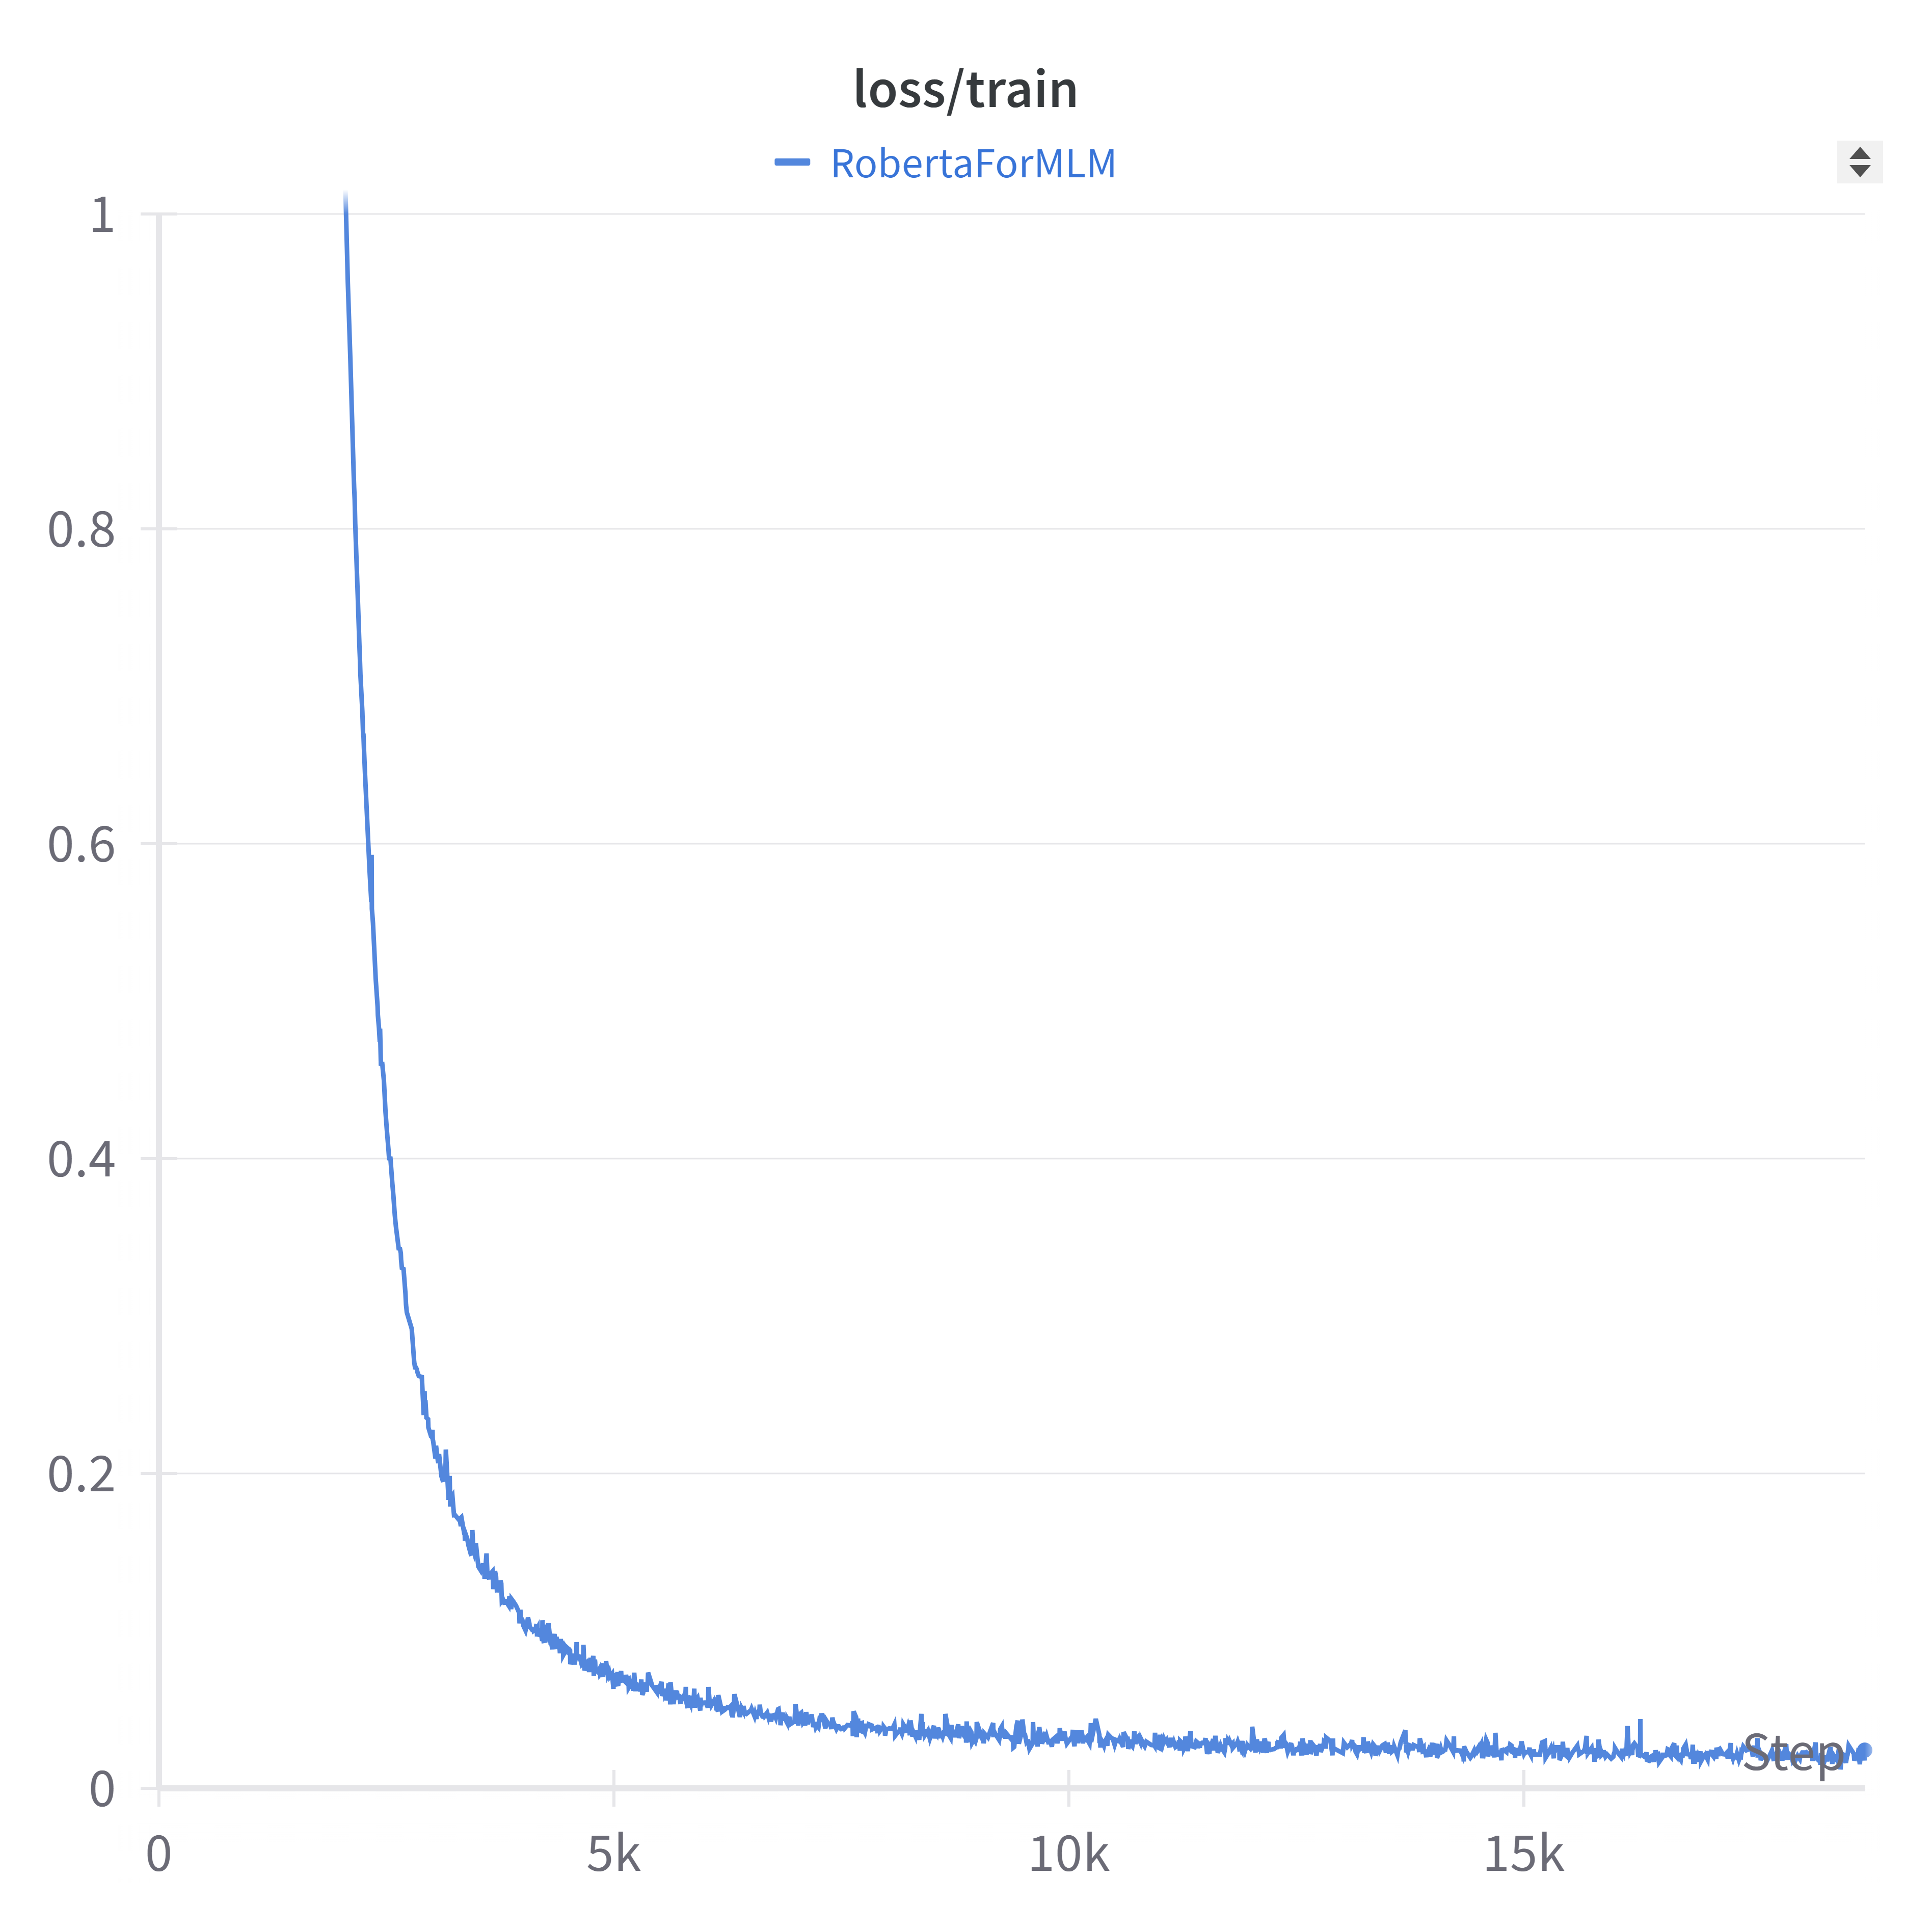
\includegraphics[width =  \textwidth ]{Bachelor-Thesis-Template/images/roberta_molclr/loss_train.png}
    \end{minipage}%
    \begin{minipage}{0.5\textwidth}
        \centering
        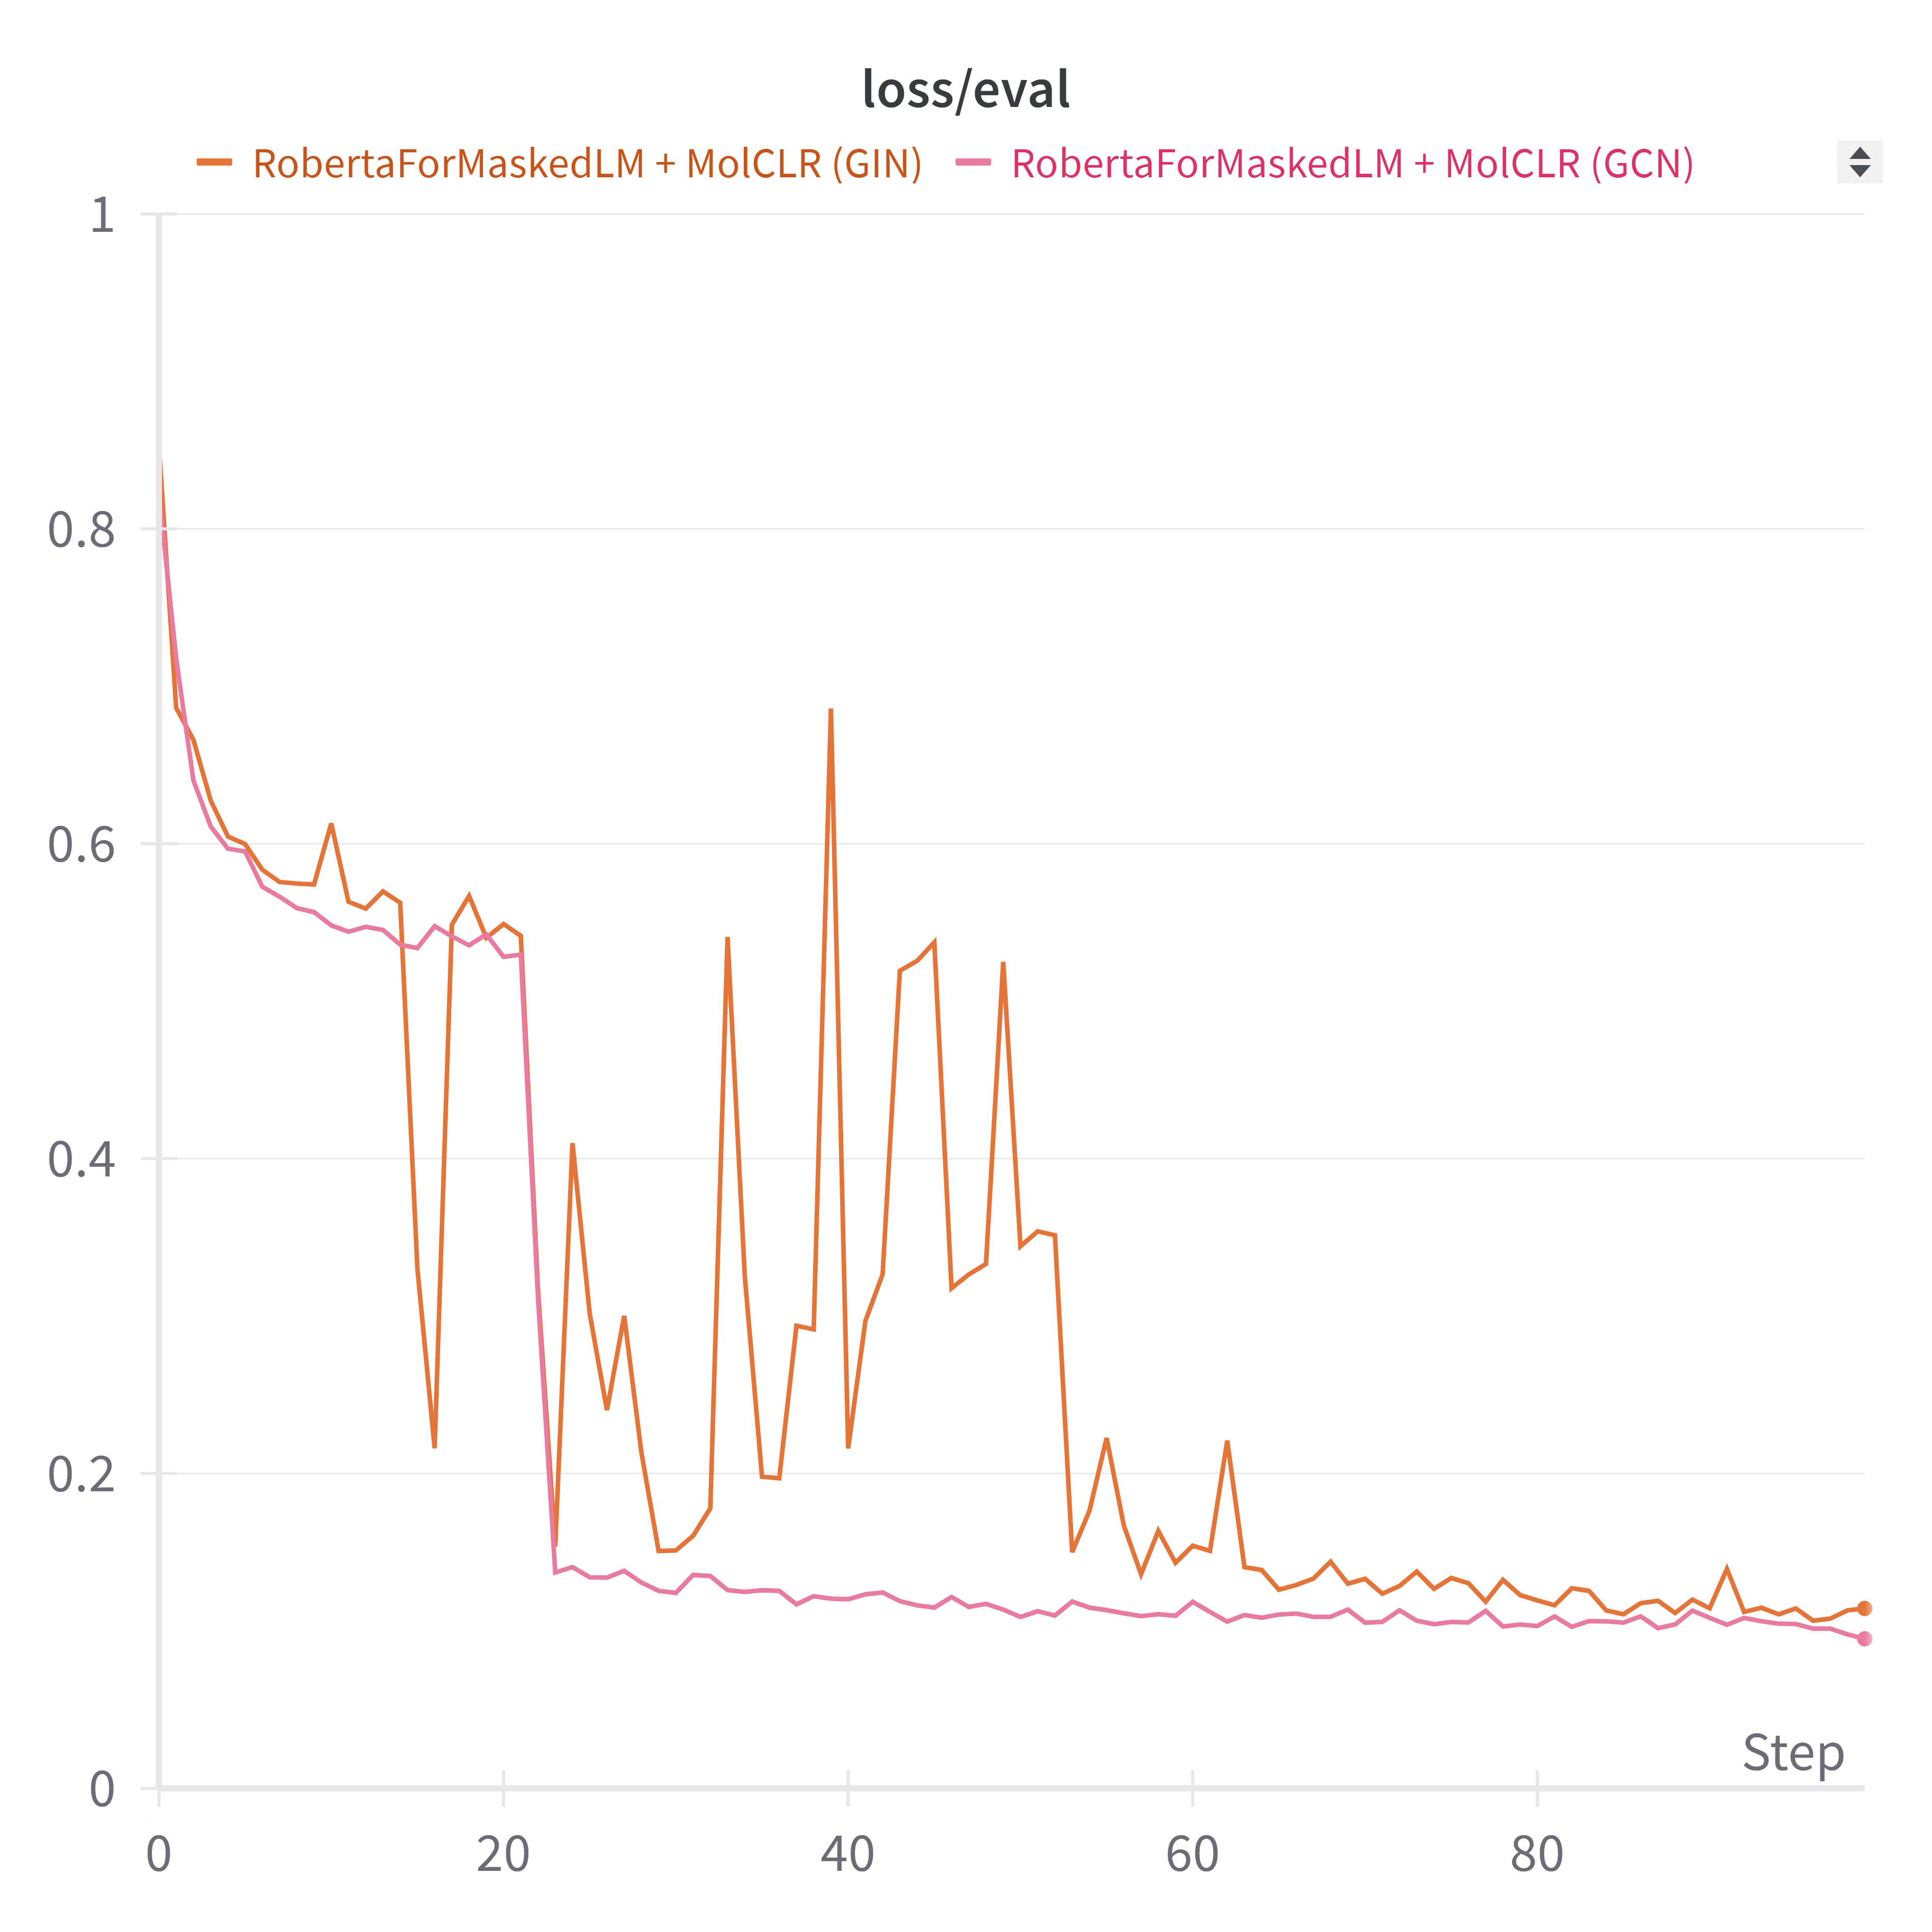
\includegraphics[width =  \textwidth ]{Bachelor-Thesis-Template/images/roberta_molclr/loss_eval.png}
    \end{minipage}%

    \newline
    \begin{minipage}{0.5\textwidth}
      \centering
    \textbf{(a)}
    \end{minipage}%
    \begin{minipage}{0.5\textwidth}
    \centering
    \textbf{(b)}
    \end{minipage}%
    
    \caption{\small Графики общей функций потерь в baseline-моделе: (a) train, (b) validation}
    \label{fig:loss_bimodal}
\end{figure}

Обе кривые на графике (a) рисунка \ref{fig:loss_bimodal} демонстрируют типичное поведение функции потерь в процессе обучения: быстрое уменьшение в начале, когда происходит основное обучение, за которым следуют более мелкие колебания и в конечном итоге стабилизация, по мере сходимости модели к оптимальным параметрам.

Красная линия, соотвествующая модели с графовой GIN, показывает резкое снижение потерь с начального значения в течение первых нескольких эпох, после чего следуют колебания с уменьшающейся амплитудой по мере продвижения вдоль шагов, в конечном итоге выравниваясь.

Оранжевая линия, соотвествующая модели с графовой GCN, также показывает начальное резкое снижение значений потерь, но с меньшими колебаниями по сравнению с красной линией, и далее она уменьшается более стабильно, приближаясь к своей асимптоте.

График валидации (b) демонстрирует аналогичные изменения для обоих конфигураций модели, что характеризует успешное проведение эксперимента и качественное обучение полученной модели.

Далее, на рисунках \ref{fig:roberta_loss_bimodal}, \ref{fig:molclr_loss_bimodal} и \ref{fig:bimodal_loss_bimodal} представлены графики функций потерь RoBERTa, MolCLR и бимодальной функции потерь в baseline-модели соответсвенно. Графики показаны при обучении модели (a) и при валидации (b), а также для двух вариантов графовой модели GCN и GIN. График междумодельной loss-функции отнормирован для наглядности.


\begin{figure}[h]
    \begin{minipage}{0.5\textwidth}
        \centering
        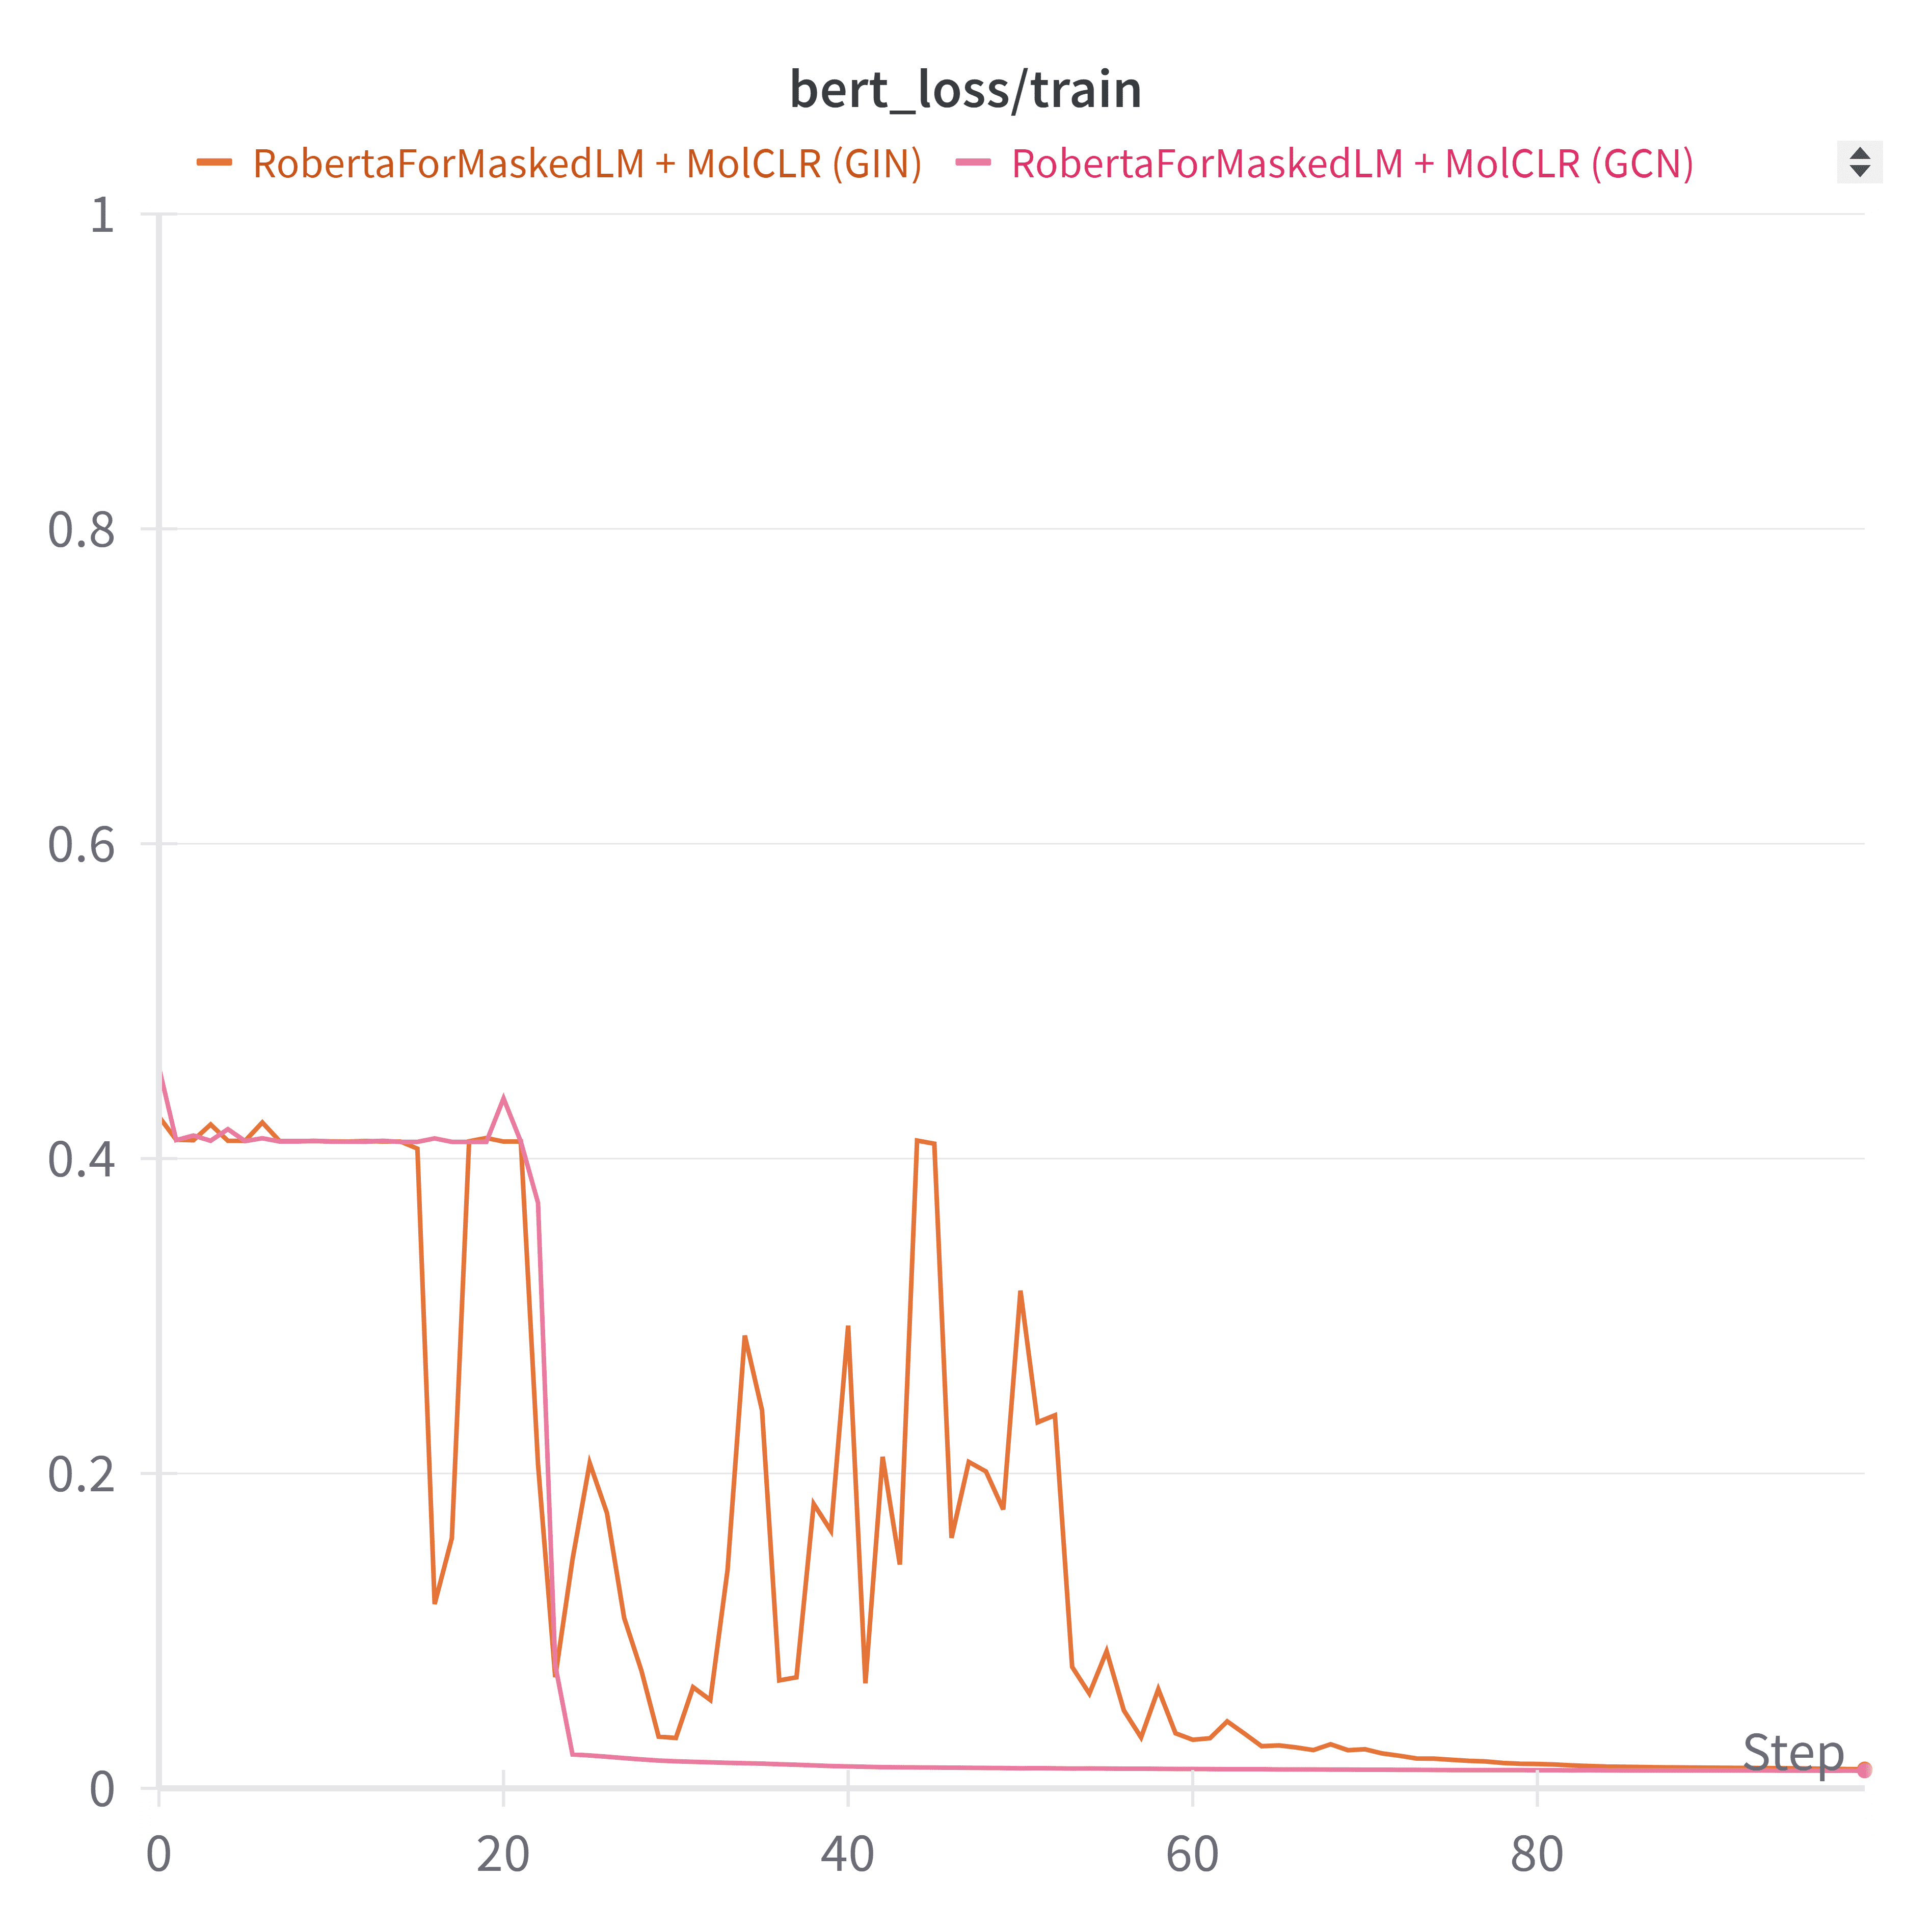
\includegraphics[width =  \textwidth ]{Bachelor-Thesis-Template/images/roberta_molclr/bert_loss_train.png}
    \end{minipage}%
    \begin{minipage}{0.5\textwidth}
        \centering
        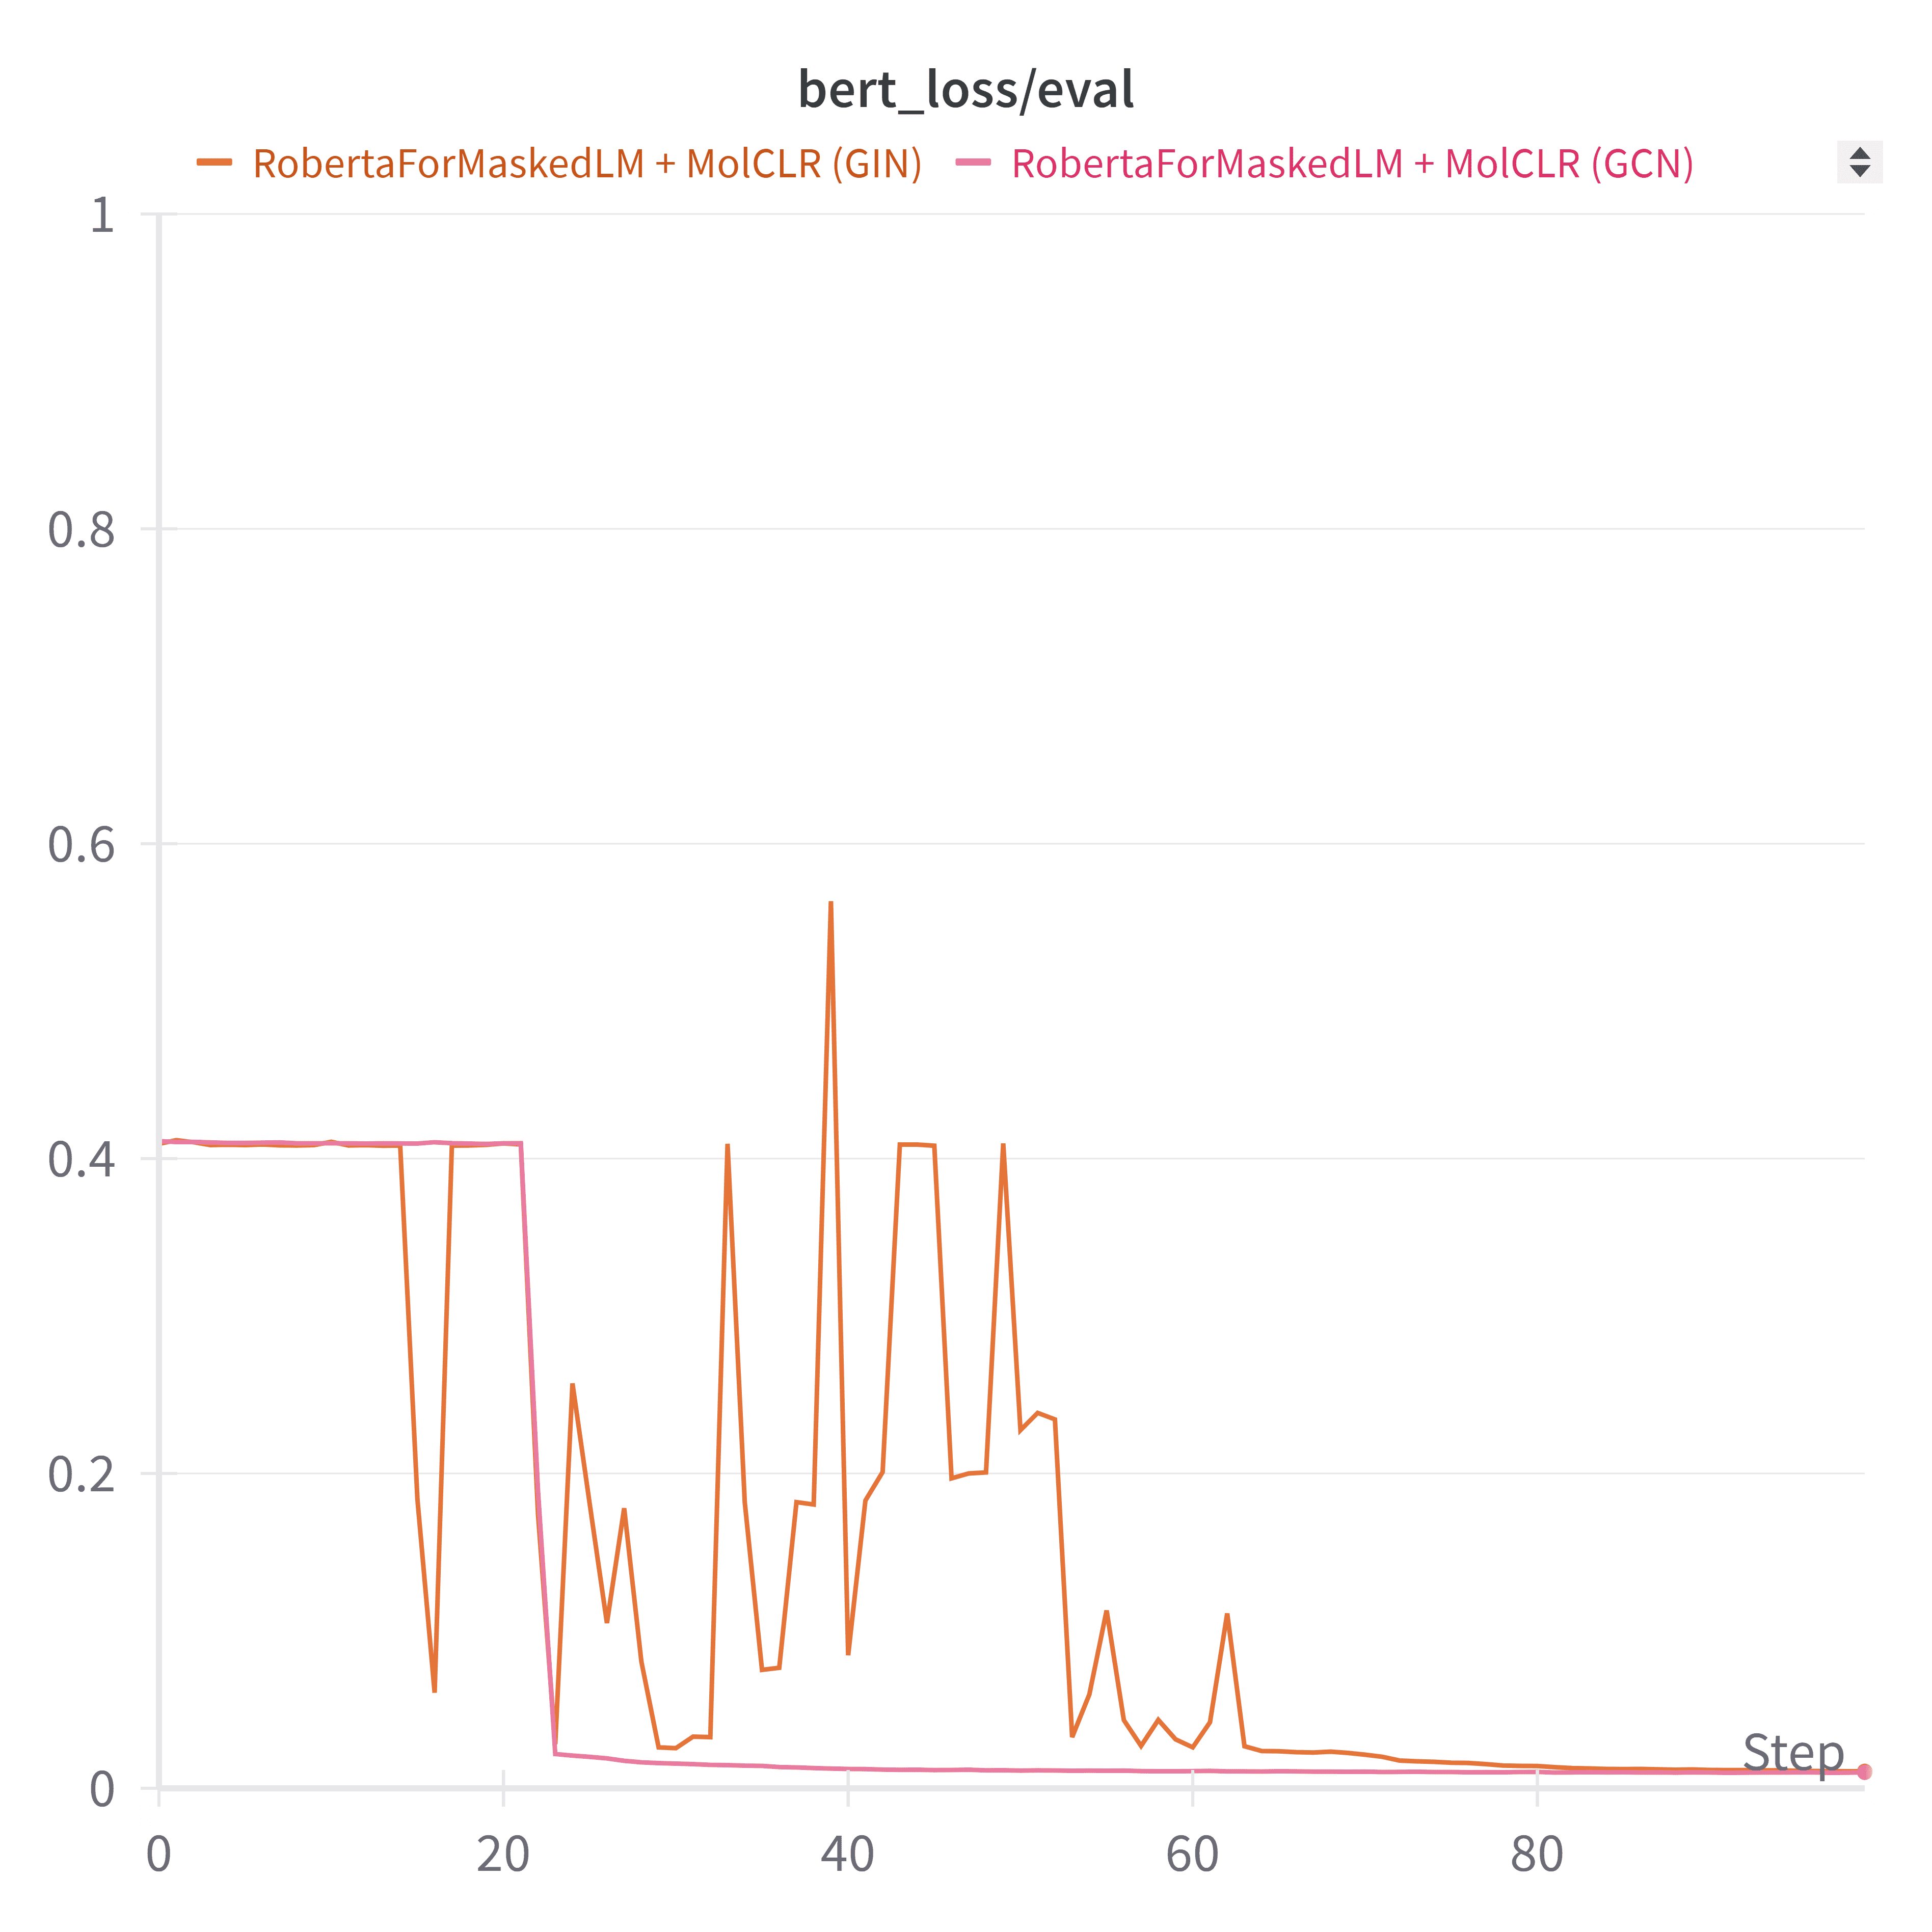
\includegraphics[width =  \textwidth ]{Bachelor-Thesis-Template/images/roberta_molclr/bert_loss_eval.png}
    \end{minipage}%

    \newline
    \begin{minipage}{0.5\textwidth}
      \centering
    \textbf{(a)}
    \end{minipage}%
    \begin{minipage}{0.5\textwidth}
    \centering
    \textbf{(b)}
    \end{minipage}%
    
    \caption{\small Графики функций потерь RoBERTa в baseline-модели: (a) train, (b) validation}
    \label{fig:roberta_loss_bimodal}
\end{figure}

Как видно на графике \ref{fig:roberta_loss_bimodal}, функция потерь RoBERTa играет основную роль в общей функции потерь, поскольку она отражает эффективность модели RoBERTa в предсказании маскированных токенов в молекулярных отпечатках ECFP. Оптимизация этой функции потерь ведет к улучшению качества эмбеддингов, получаемых от модели RoBERTa, что, в свою очередь, влияет на общую функцию потерь и эффективность всей модели.

На данных рисунках видны резкие измения графика, которые могли быть вызваны некорректно подобранным шагом обучения. Эти колебания характеризуются резкими всплесками и спадами, что отражает итеративный процесс оптимизации в процессе обучения. GCN, демонстрирует схожую динамику, но с меньшей степенью волатильности.

\begin{figure}[h]
    \begin{minipage}{0.5\textwidth}
        \centering
        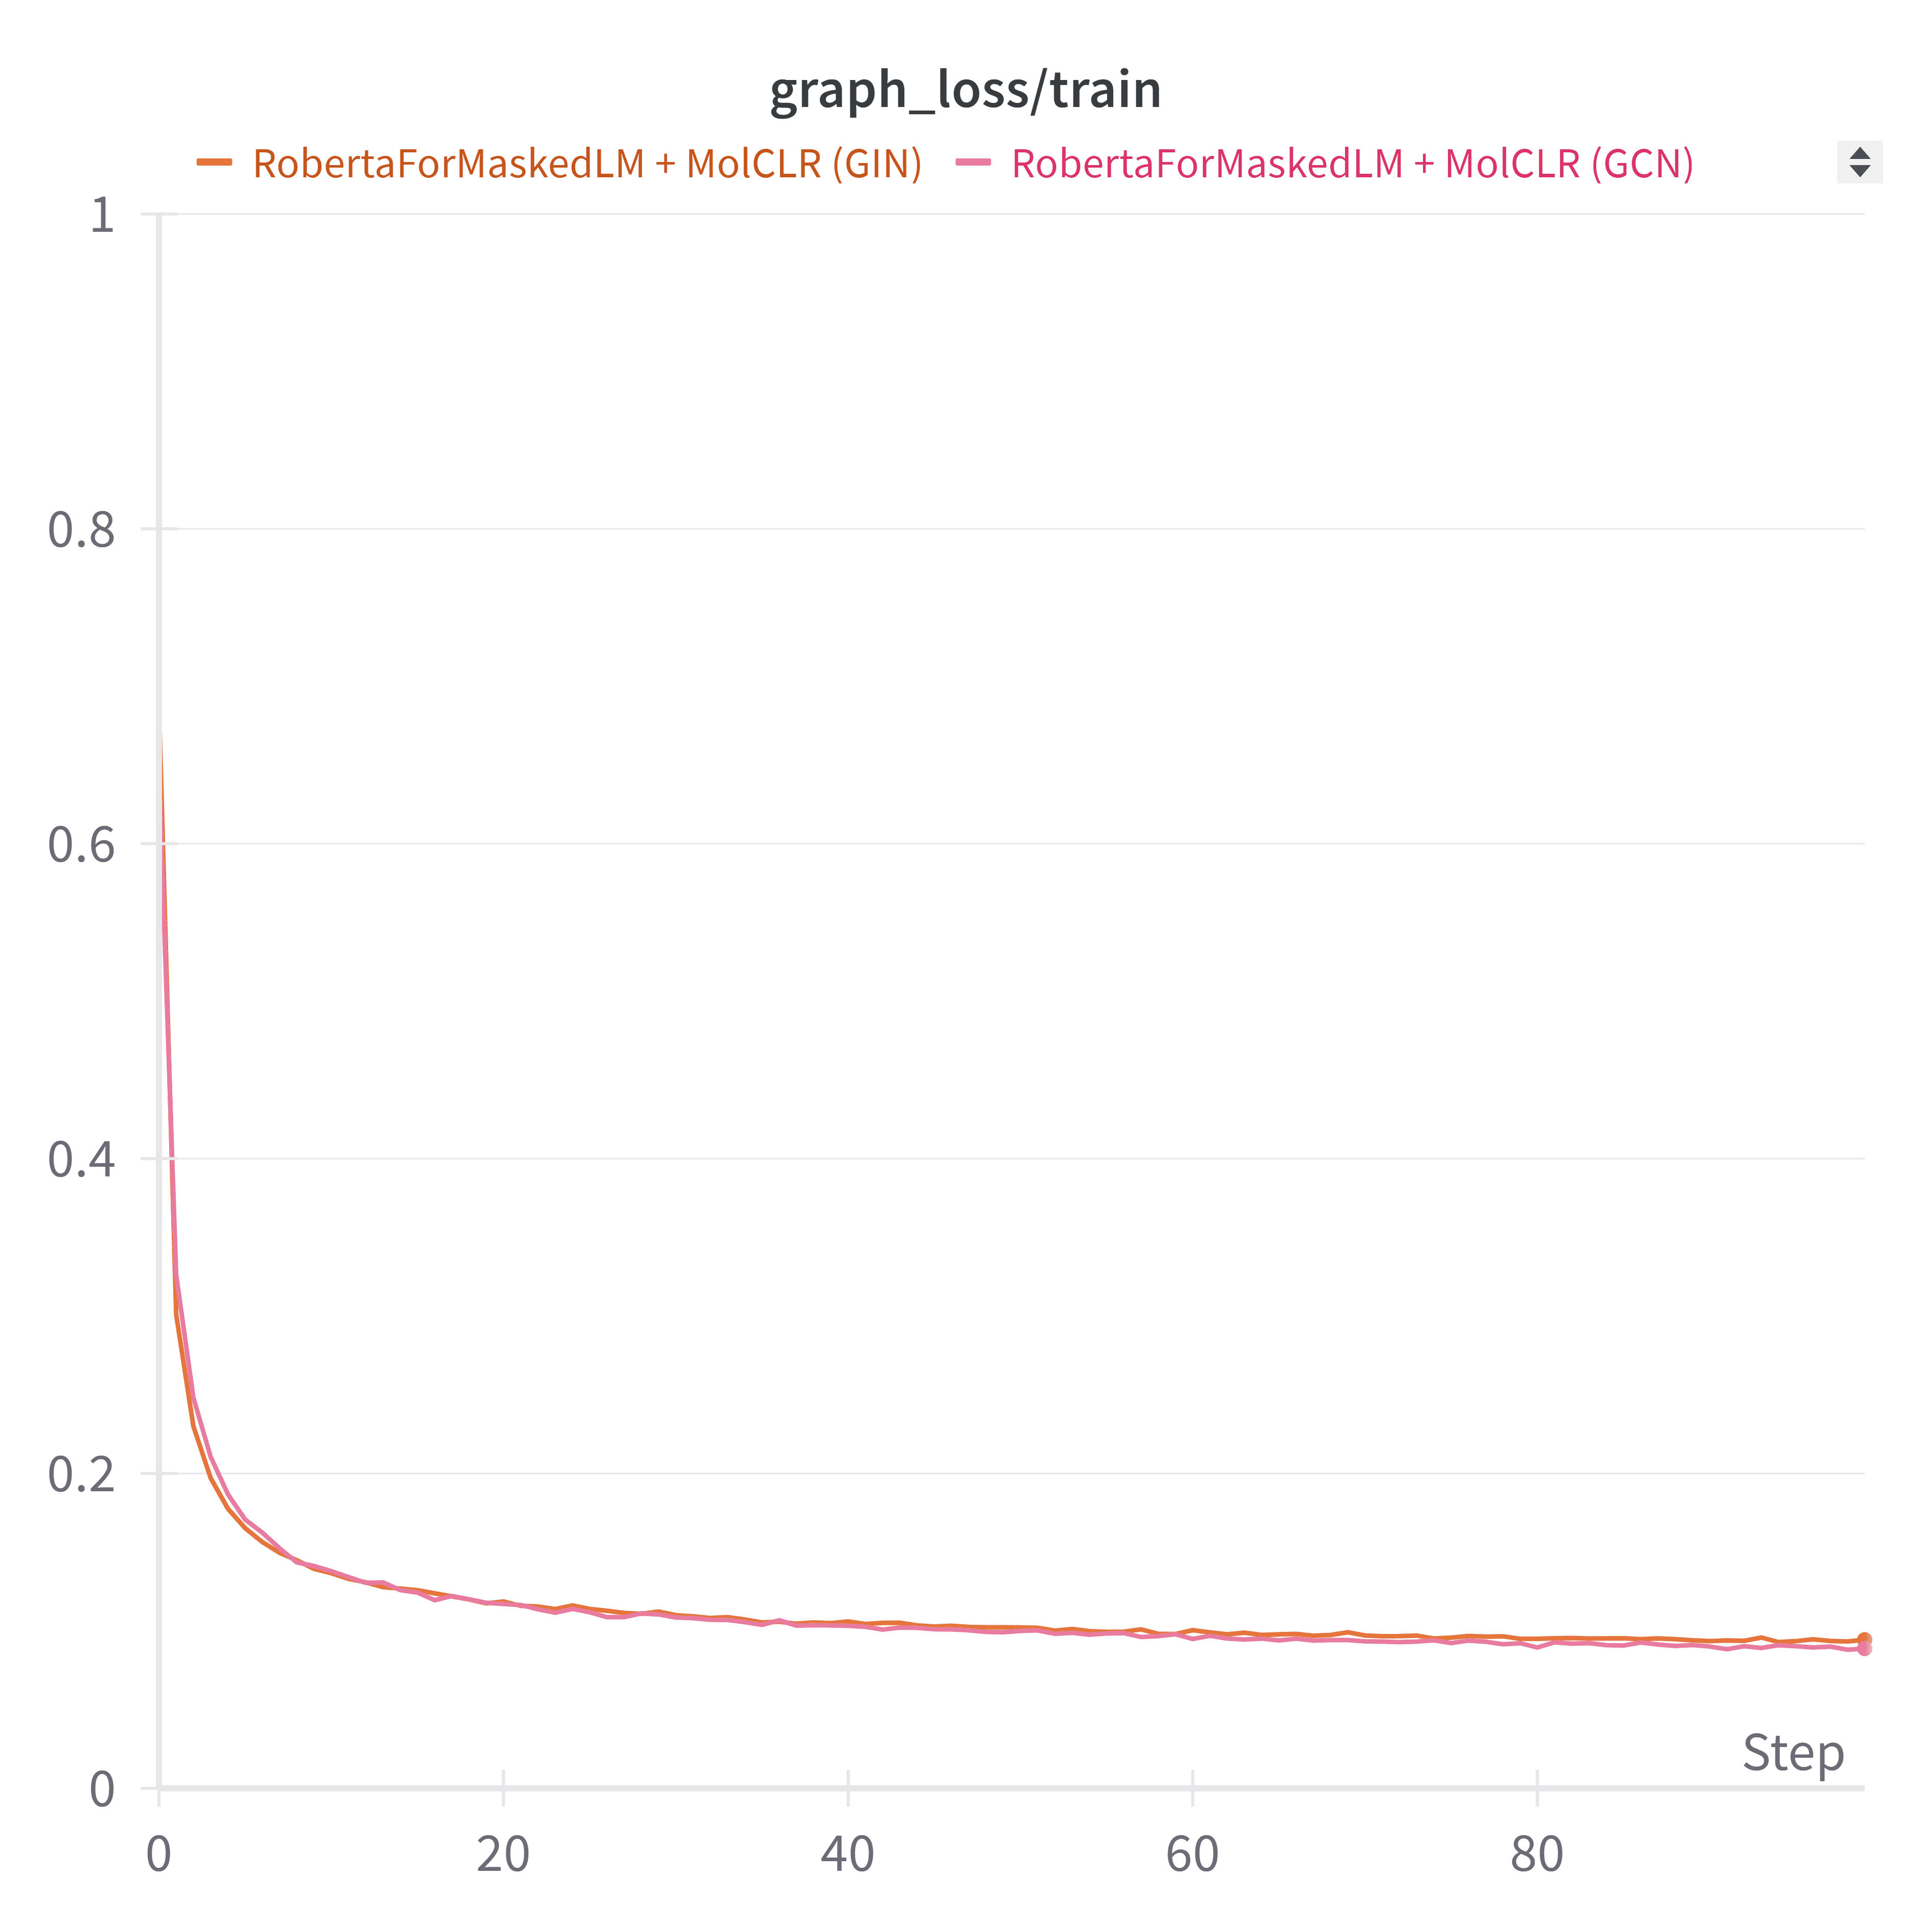
\includegraphics[width =  \textwidth ]{Bachelor-Thesis-Template/images/roberta_molclr/graph_loss_train.png}
    \end{minipage}%
    \begin{minipage}{0.5\textwidth}
        \centering
        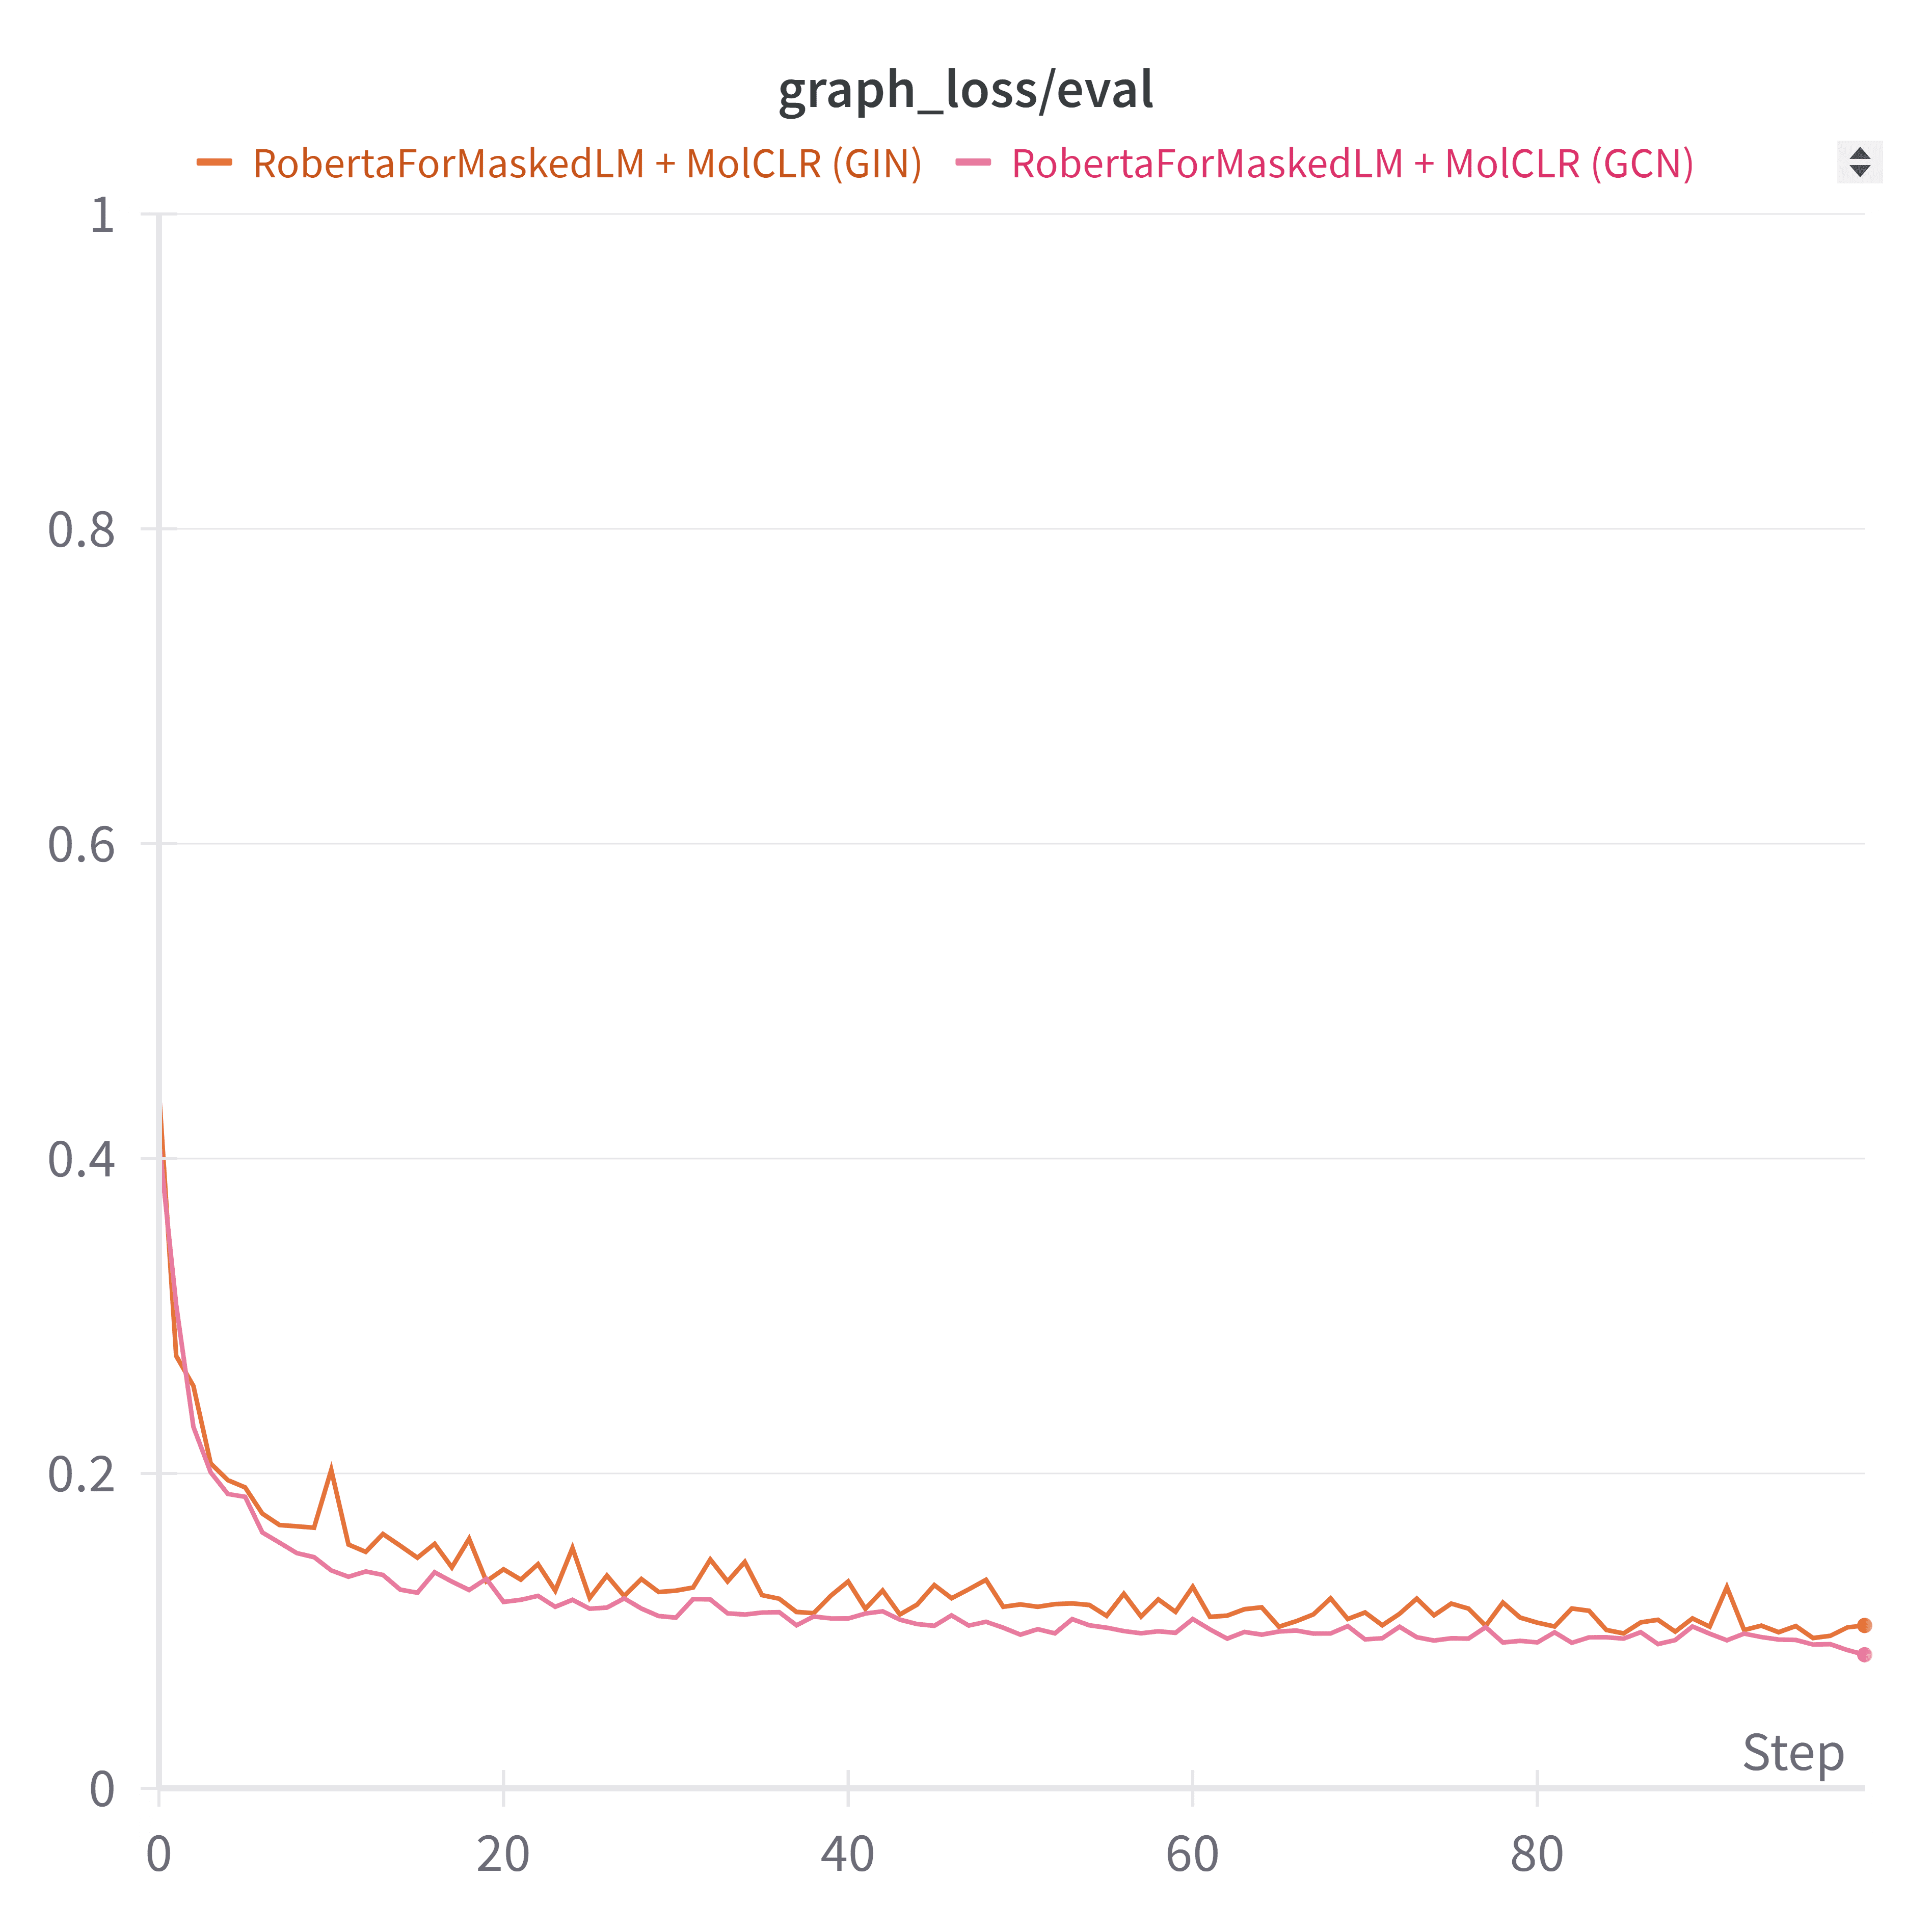
\includegraphics[width =  \textwidth ]{Bachelor-Thesis-Template/images/roberta_molclr/graph_loss_eval.png}
    \end{minipage}%

    \newline
    \begin{minipage}{0.5\textwidth}
      \centering
    \textbf{(a)}
    \end{minipage}%
    \begin{minipage}{0.5\textwidth}
    \centering
    \textbf{(b)}
    \end{minipage}%
    
    \caption{\small Графики функций потерь MolCLR в baseline-модели: (a) train, (b) validation}
    \label{fig:molclr_loss_bimodal}
\end{figure}
Функция потерь MolCLR также играет важную роль в общей функции потерь, поскольку она отражает эффективность модели MolCLR в генерации эмбеддингов графов молекул. Это подтверждается графиком \ref{fig:molclr_loss_bimodal}, где на обучении и валидации обе модели демонстрируют схожую динамику уменьшения функции потерь. Это указывает на то, что обе модели успешно обучаются, улучшают свою производительность с течением времени, однако быстро достигают "плато".

\begin{figure}[h]
    \begin{minipage}{0.5\textwidth}
        \centering
        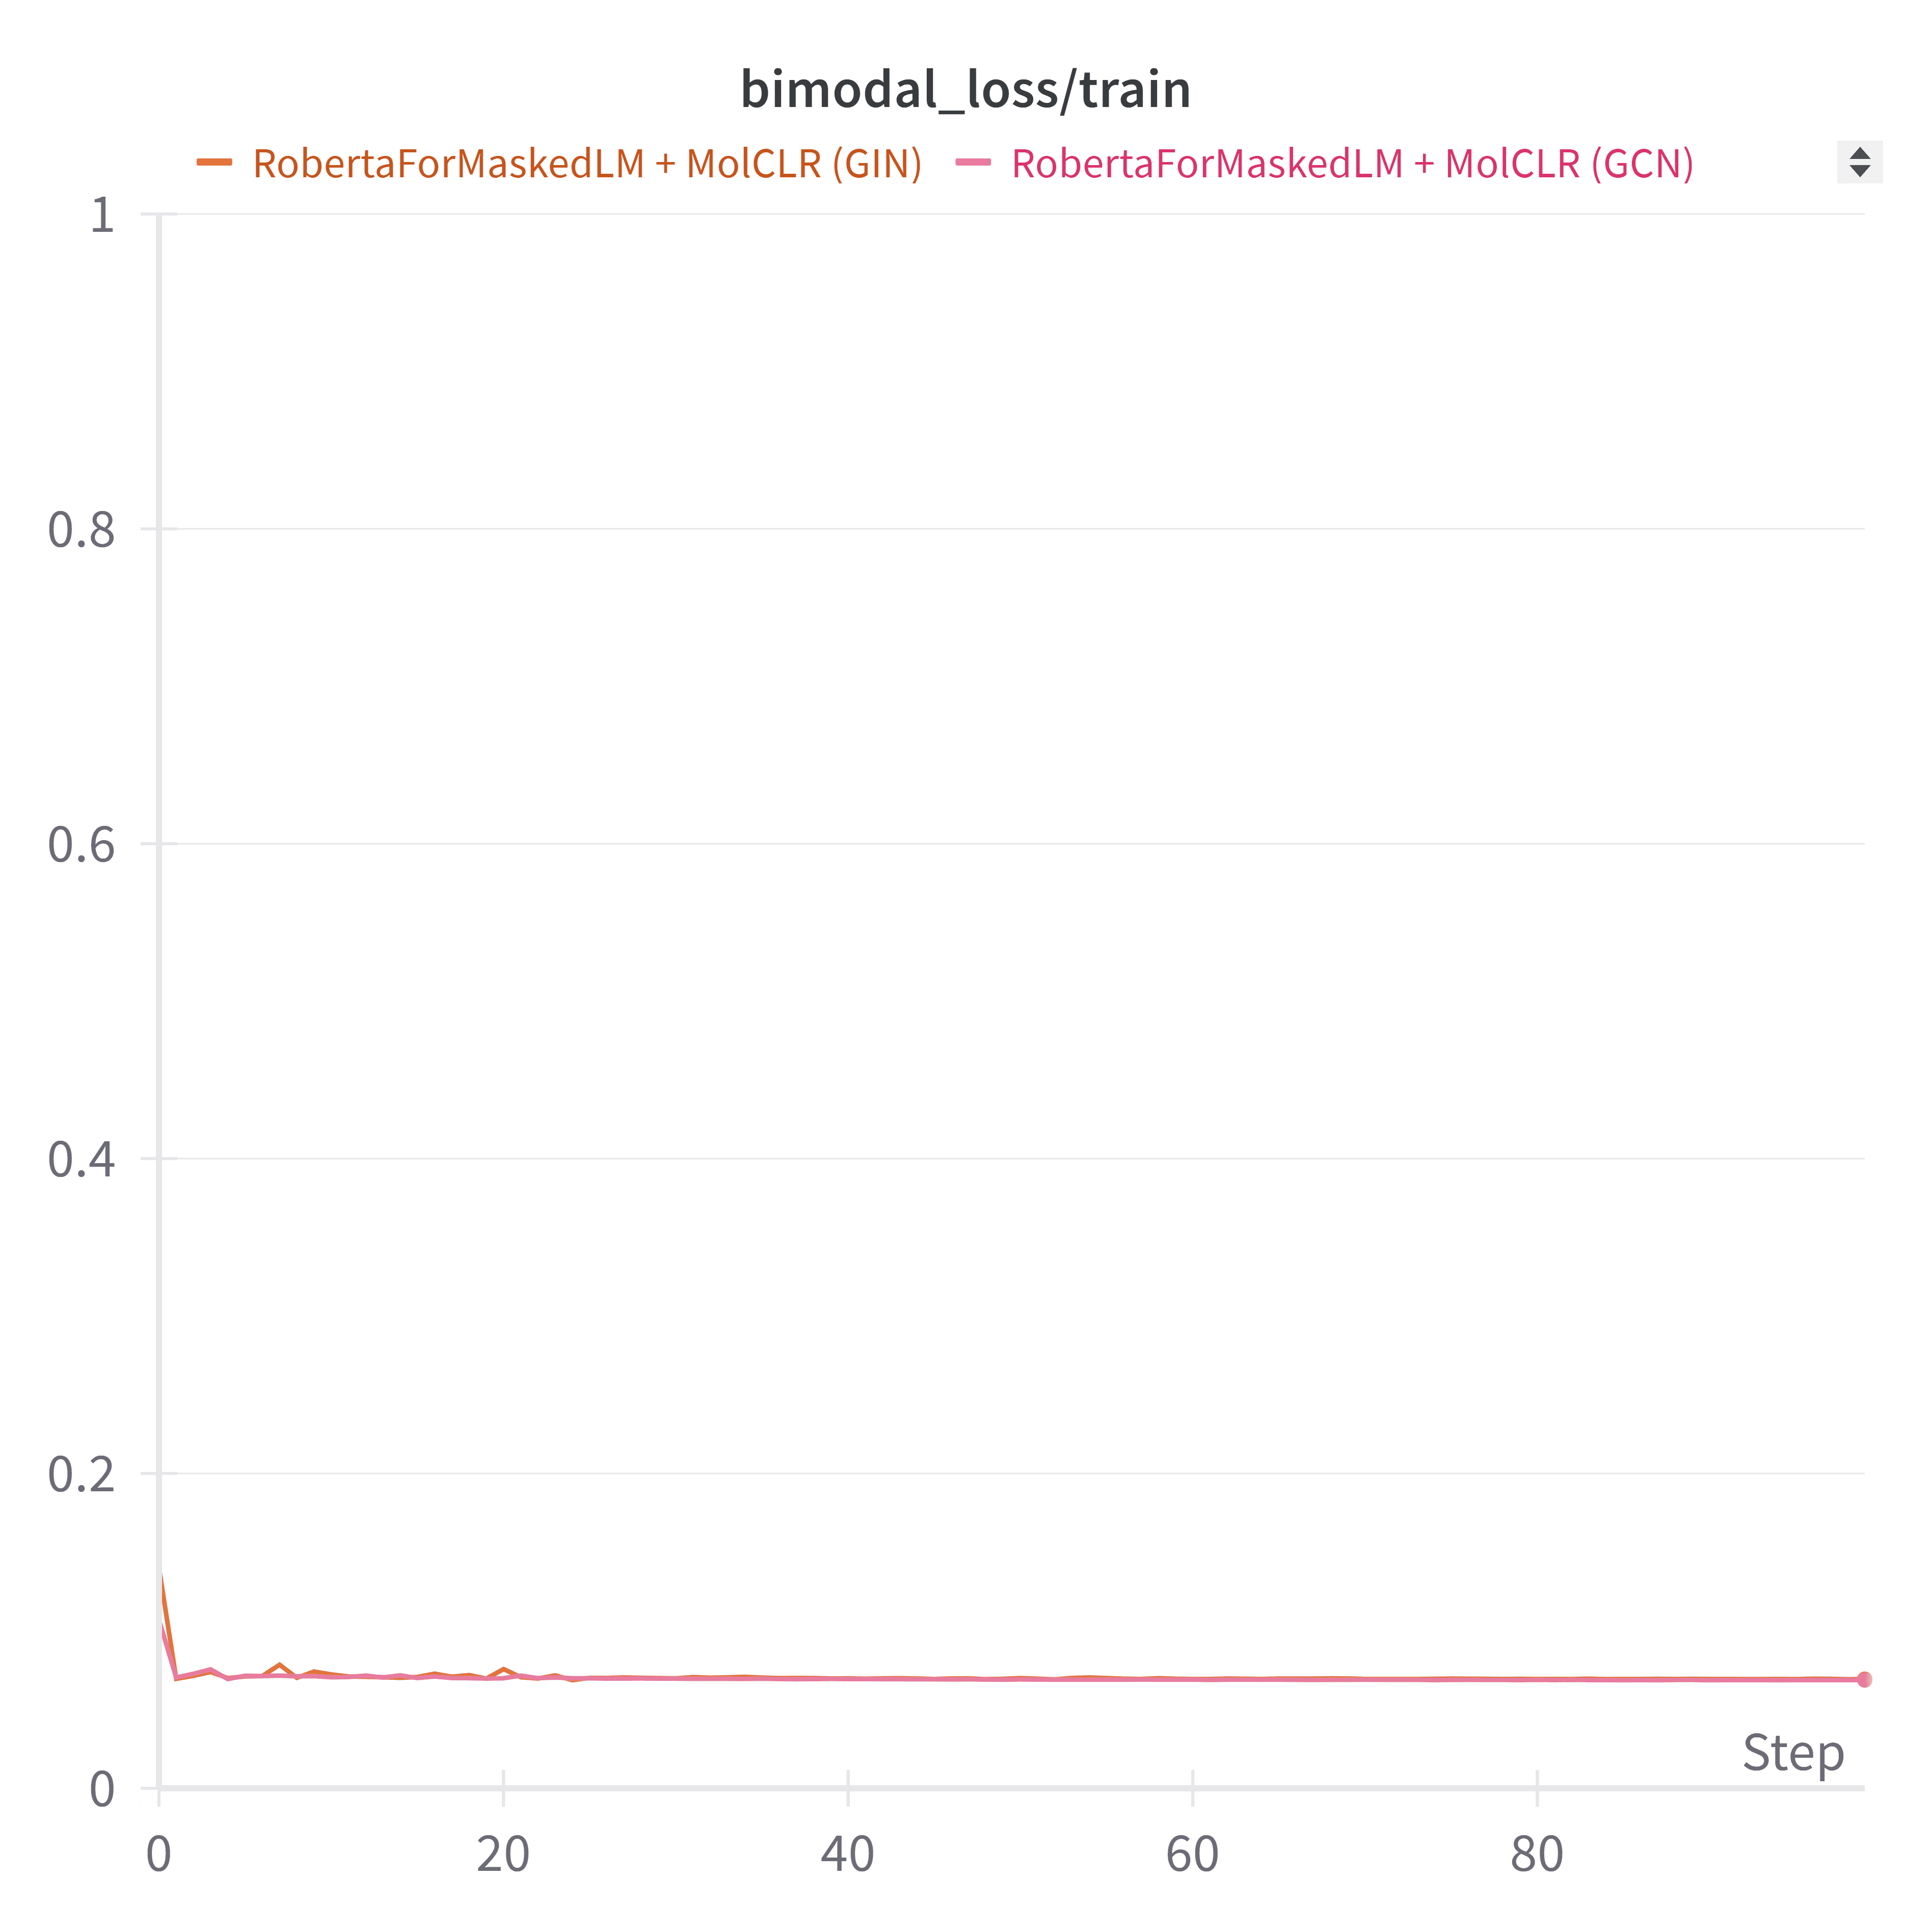
\includegraphics[width =  \textwidth ]{Bachelor-Thesis-Template/images/roberta_molclr/bimodal_loss_train.png}
    \end{minipage}%
    \begin{minipage}{0.5\textwidth}
        \centering
        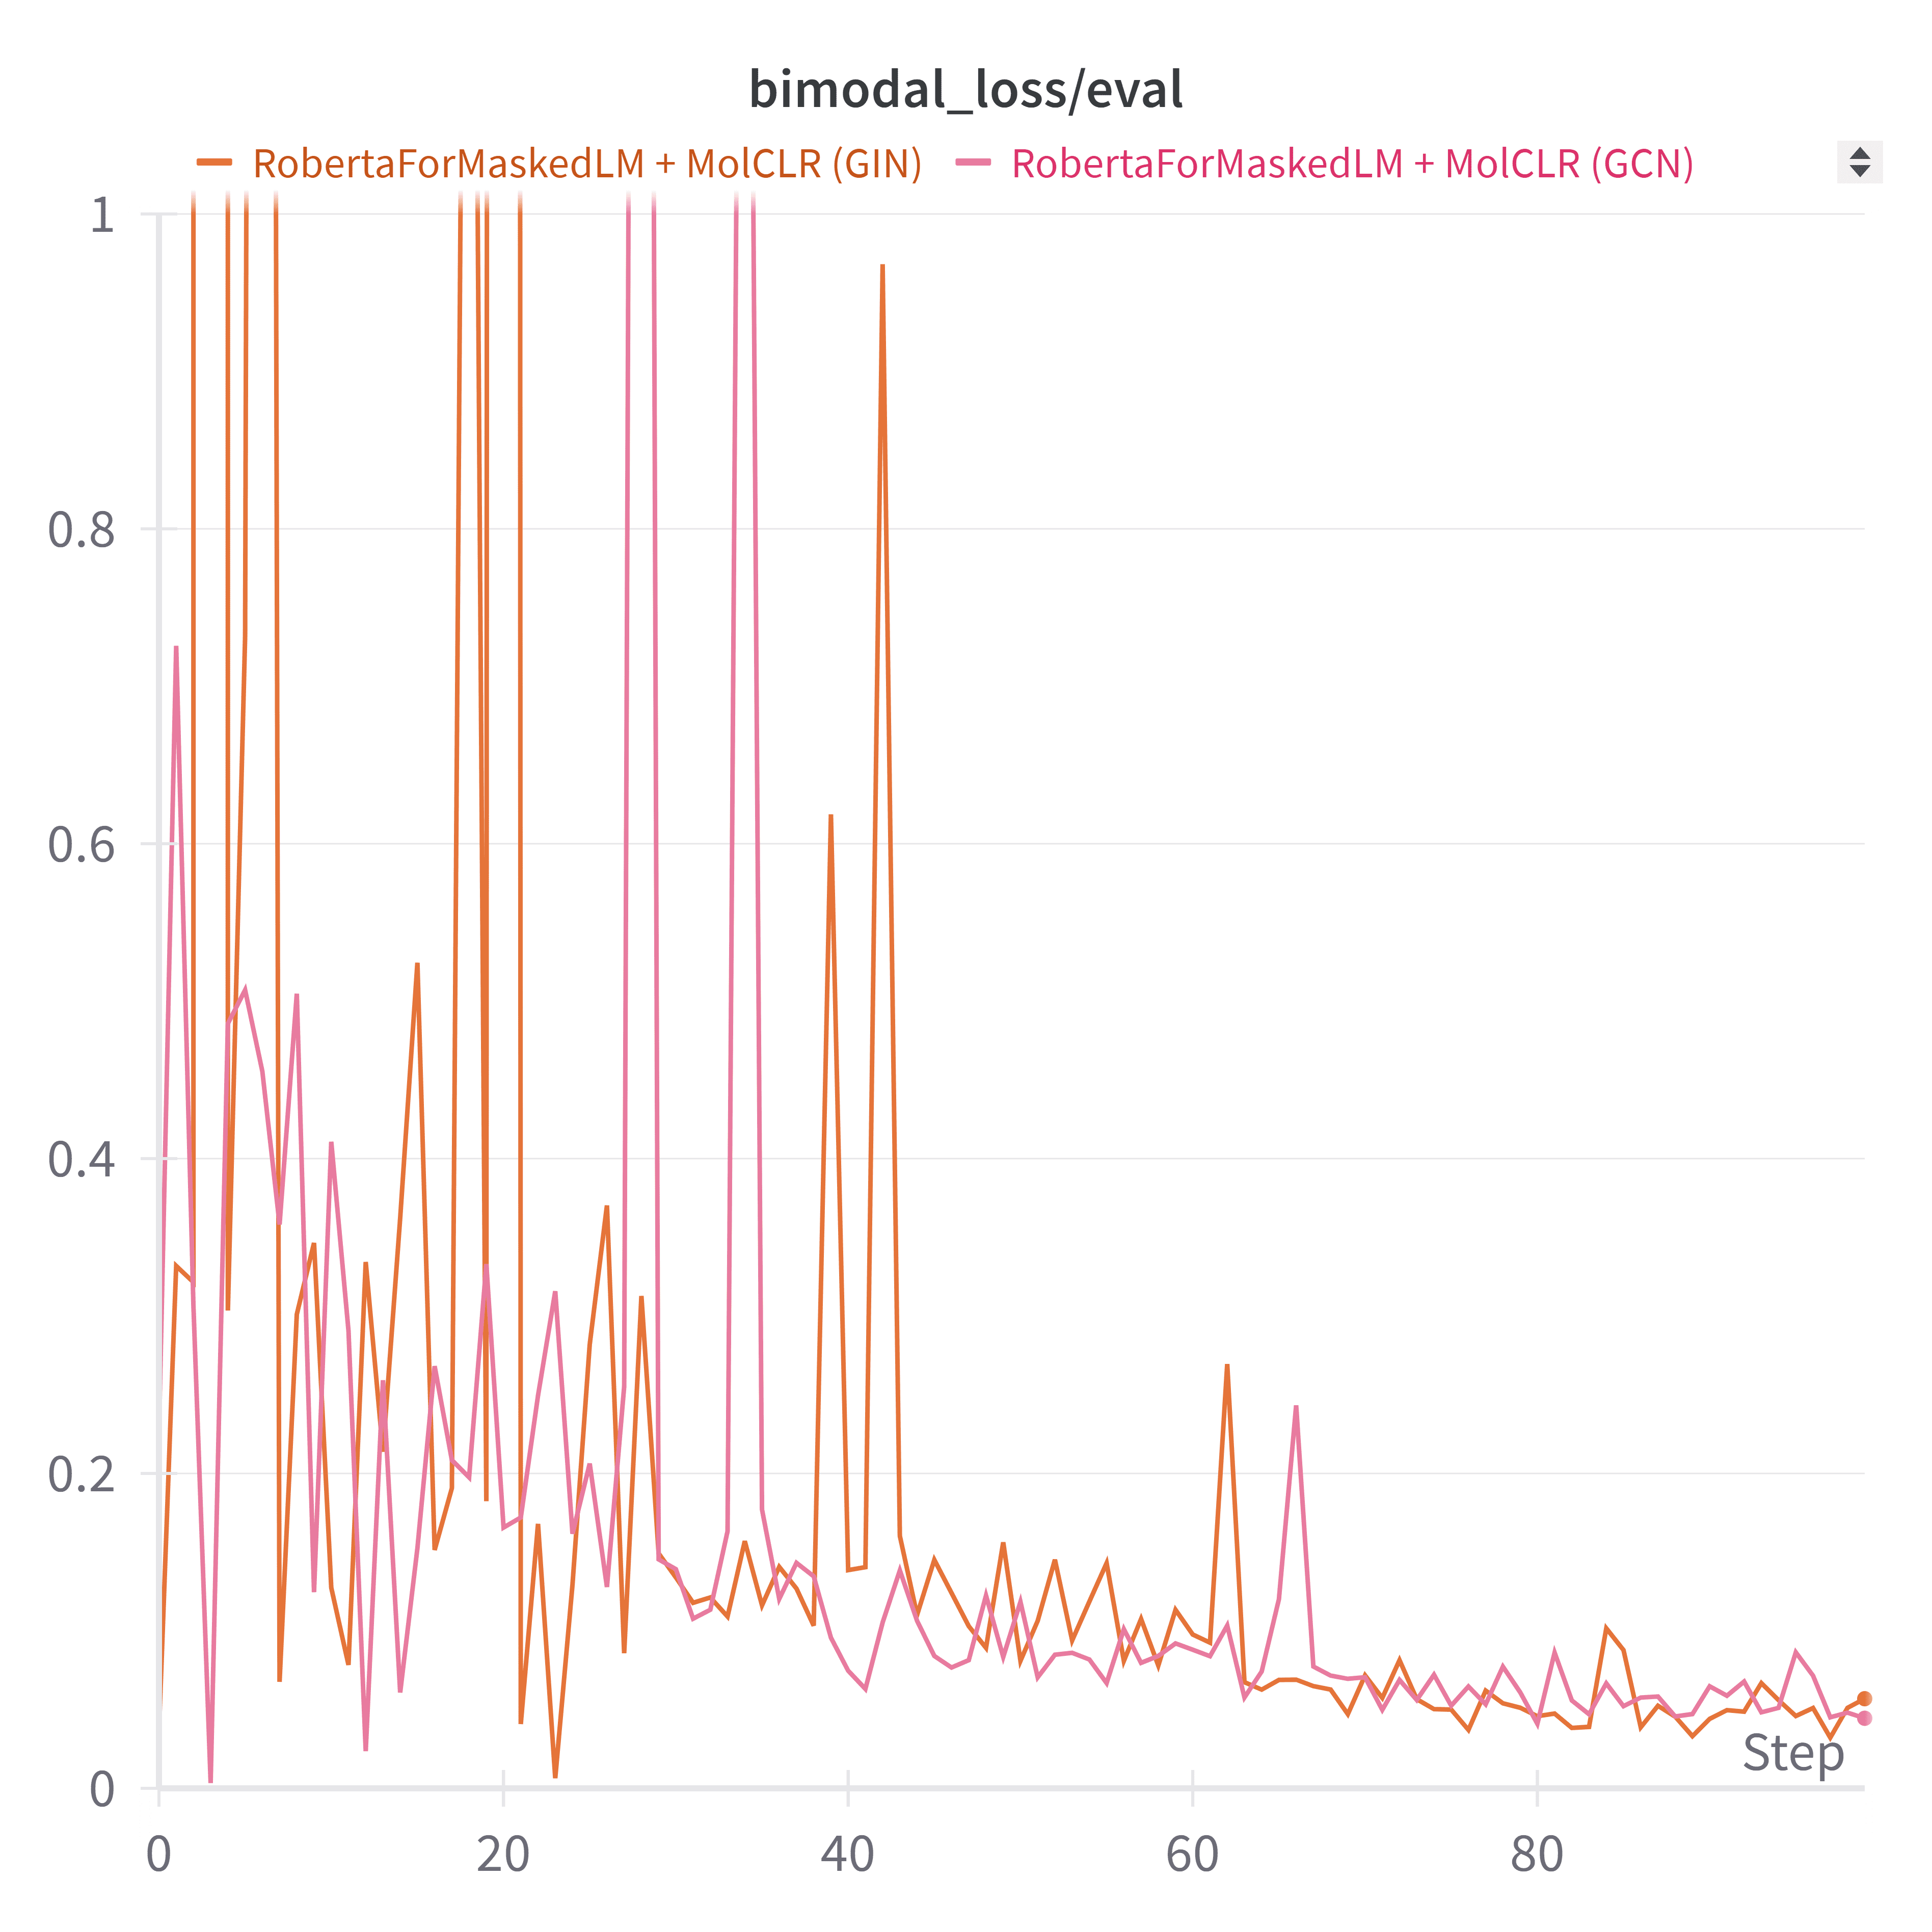
\includegraphics[width =  \textwidth ]{Bachelor-Thesis-Template/images/roberta_molclr/bimodal_loss_eval.png}
    \end{minipage}%

    \newline
    \begin{minipage}{0.5\textwidth}
      \centering
    \textbf{(a)}
    \end{minipage}%
    \begin{minipage}{0.5\textwidth}
    \centering
    \textbf{(b)}
    \end{minipage}%
    
    \caption{\small Графики бимодальной функций потерь в baseline-модели: (a) train, (b) validation}
    \label{fig:bimodal_loss_bimodal}
\end{figure}

На представленном выше графике рисунка \ref{fig:bimodal_loss_bimodal} отображены динамики бимодальной функции потерь на этапе обучени и валидации. Данная функция является косинусоидальным расстоянием между внутренними представлениями RoBERTa и MolCLR. Начальное значение (расстояние между случайными эмбеддингами) равно приблизительно 1, однако оно быстро сходится к числу, сильно меньше 0.1. Поэтому стоит отметить, что значения функции потерь на этом графике умножены на 100 для наглядности, поскольку исходные значения \texttt{bimodal\_loss} получаются слишком близкими к нулю.

Несмотря на то, что функция потерь между двумя моделями является важной составляющей общей функции потерь, ее вклад в общую функцию потерь оказывается относительно небольшим. Полученные результаты свидетельствует о высокой степени согласованности эмбеддингов, получаемых от моделей RoBERTa и MolCLR, а также достаточно быстрой сходимости данной функции похожести эмбеддингов при обучении.

\textbf{Про коэффиценты общего loss:}
В ходе экспериментов была предпринята попытка установить коэффициенты $\alpha$, $\beta$, $\gamma$ обратно пропорциональными начальным значениям соответствующих функций потерь. Однако, как показали результаты, такой подход приводит к эффекту, аналогичному случаю, когда все коэффициенты равны 1. Это может быть связано с тем, что обратная пропорциональность начальных значений потерь приводит к нормализации вклада каждой компоненты потери в общую потерю. В результате, каждая компонента потери вносит примерно одинаковый вклад в общую потерю.

Таким образом, для дальнейшего анализа были выбраны результаты, полученные при $\alpha = \beta = \gamma = 1.0$. В этом случае все функции потерь вносят одинаковый вклад в общую функцию потерь.



\newpage

